\newpage

\section{Porównanie wybranych algorytmów i próby optymalizacji} \label{sec:testing}

W ramach pracy dyplomowej podjęte zostały próby usprawnienia i optymalizacji różnych aspektów projektu. Testowany był wpływ rozdzielczości danych SRTM terenu na dokładność odwzorowania modelu oraz czas ich przetwarzania. Podjęta została próba optymalizacji procesu poprzez odrzucenie niepotrzebnych w danym momencie próbek terenu, zmniejszając przetwarzaną ich liczbę. Z powodu mnogości dostępnych metod obliczania odległości między punktami geograficznym, zostały one przebadane ze względu na dokładność, a także na czas wykonania potrzebnych obliczeń. Skuteczność dopasowania obrazów binarnych zawierających kontury gór na modelu terenu oraz na zdjęciu rzeczywistym wydaje się kluczowym czynnikiem wpływającym na jakość rozwiązania. Mając to na uwadze zostały przetestowane i porównane metody dopasowania na podstawie szablonu oraz na podstawie cech. Przeprowadzono również próbę optymalizacji tych klasyfikatorów pod względem jakościowym poprzez zastosowanie operacji morfologicznej dylacji oraz zbadano jej wpływ na ten aspekt. Na koniec przeprowadzono profilowanie procesu rozpoznawania szczytów wykonywanego na platformie testowej, które pozwoliło wyłapać ewentualne błędy implementacyjne oraz tzw. wąskie gardła zaproponowanego procesu. Dzięki temu wykryta została możliwość usprawnienia systemu poprzez lepsze wykorzystanie pamięci podręcznej procesora. 

W przypadku testów i porównań złożoności czasowej rozwiązań badania były przeprowadzane przy pomocy trzech różnych urządzeń z system Android. Były one zróżnicowane pod względem wydajnościowym, jak i lat produkcji. Wykorzystane były urządzenia marki Huaweii: Mate 20 Lite, P30 Pro oraz Mate 50 Pro. Przedstawione zostały w kolejności od najmniejszej mocy obliczeniowej do największej. 


\subsection{Wpływ rozdzielczości danych SRTM na dokładność odwzorowania terenu} \label{sec:rozdzielczosc_srtm}

Opisane wcześniej dane SRTM w wersji podstawowej $1^{\prime\prime}$ zawierają $12 \; 967 \; 201$ wartości na jedną kratkę ($3601 \textrm{x} 3601$) siatki geograficznej. Natomiast, w przypadku rozdzielczości~$3^{\prime\prime}$ próbek jest już tylko $1 \; 442 \; 401$ ($1201 \textrm{x} 1201$). Jest to prawie $90\%$ mniej wpisów.

Mimo, że rzadsze próbkowanie zawiera dziewięciokrotnie mniej danych, to jednak dla problemu detekcji szczytów górskich, dokładne odwzorowanie terenu nie zawsze musi być aż tak znaczące. Na rzeczywistych zdjęciach pasma górskie mogą być oddalone nawet o kilkanaście czy kilkadziesiąt kilometrów, więc ich szczegółowość nie będzie duża. Tak samo, trójwymiarowy model terenu w zależności od rozdzielczości danych, będzie różnić się tylko detalami. Odwzorowanie pasm górskich zostanie mimo to zachowane. 



Ze względu na dużą różnice w liczbie danych, porównane zostały modele generowane z~wykorzystaniem obu rozdzielczości. Badanie polegało na subiektywnej ocenie dokładności krawędzi pasm renderowanego terenu w wybranych lokalizacjach geograficznych.

Przykładowe porównanie modeli pokazane zostało na rysunku \ref{fig:render-resolution-comp}. Przedstawia on wycinki wyrenderowanych gór oddalonych w rzeczywistości o $10-20$ km. 

\begin{figure}[!h]
    \centering 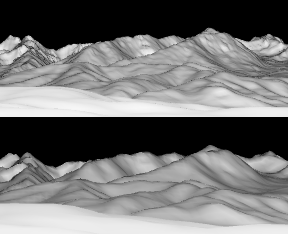
\includegraphics[width=0.65\linewidth]{img/new_compare.png}
    \caption{Porównanie generowanego terenu w zależności od rozdzielczości danych. Górny wyrenderowany model prezentuje dokładność $30$ m, dolny natomiast $90$ m.}
    \label{fig:render-resolution-comp}
\end{figure}

Na podstawie pokazanego porównania można stwierdzić, że główne kontury pasm górskich są widoczne w podobnym i dostatecznym stopniu na obu wizualizacjach. Bardziej dokładny model posiada więcej szczegółów związanych z nierównościami terenu, drobnymi pagórkami czy gwałtownymi zmianami wysokości. Na potrzeby detekcji krawędzi gór obie wizualizacje są wystarczające, ze względu na to, że pasma horyzontalne są wyraźnie widoczne. Dodatkowo, bardziej dokładne dane mogę mieć negatywny wpływ na rozpoznawanie tych elementów poprzez zwiększenie zaszumienia wizualizacji mało istotnymi konturami i zmianami odcieni terenu. 

Przeprowadzone zostało badanie wpływu rozdzielczości zbioru danych na czas generowanie trójkątów i wierzchołków modelu. Wyniki tego testu zostały przedstawione w~tabeli~\ref{tab:render-res-time-comp}. Długość trwania tych operacji w przypadku mniej dokładnego zestawu danych wyniosła około $10-12\%$ czasu potrzebnego na te same czynności wykonane przy wykorzystaniu danych o większej rozdzielczości. Dane te potwierdzają opisane rozważania teoretyczne. Każdy przypadek testowy przeprowadzony był dziesięciokrotnie, a wynik uśredniony. Rezultaty jednoznacznie pokazują znaczne zmniejszenie okresu potrzebnego na przetworzenie wejściowych danych dotyczących terenu, co może mieć istotne znaczenie przy komforcie użytkowania takiego projektu. Dane wczytywane i~przygotowywane są w czasie ładowania aplikacji, a nie jej działania, dlatego wpływ może mieć głównie na subiektywne odczucia podczas jej używania, a nie na wydajności w~kontekście pracy w~czasie rzeczywistym. 

\begin{table}[!h]
  \centering
  \caption{Porównanie czasu generowania wierzchołków i trójkątów w zależności od rozdzielczości danych SRTM.}
  \begin{tabularx}{\linewidth}{|l|*{3}{>{\centering\arraybackslash}X|}*{3}{>{\centering\arraybackslash}X|}}
    \hline
    \begin{tabular}[c]{@{}c@{}} \\ Urządzenie \end{tabular} & \multicolumn{3}{c|}{\begin{tabular}[c]{@{}c@{}}Czas generowania\\ wierzchołków \end{tabular}} & \multicolumn{3}{c|}{\begin{tabular}[c]{@{}c@{}}Czas generowania\\ trójkątów \end{tabular}} \\
    \cline{2-7}
      & $1^{\prime\prime}$ & $3^{\prime\prime}$ & $\frac{t_{1^{\prime\prime}}}{t_{3^{\prime\prime}}}$ & $1^{\prime\prime}$ & $3^{\prime\prime}$ & $\frac{t_{1^{\prime\prime}}}{t_{3^{\prime\prime}}}$\\
    \hline
    \hline
    Mate 20 Lite & 0,3576 s & 0,0516 s & 0,1444 & 0,3330 s & 0,0364 s & 0,1095 \\
    \hline
    P30 Pro & 0,1794 s & 0,0209 s & 0,1170 & 0,2256 s & 0,0231 s & 0,1026 \\
    \hline
    Mate 50 Pro & 0,1197 s & 0,0135 s & 0,1129 & 0,1526 s & 0,0147 s & 0,0969 \\
    \hline
  \end{tabularx}
  \label{tab:render-res-time-comp}
\end{table}



Więcej danych oznacza również zwiększenie zapotrzebowania na zasoby pamięci celem przechowania znacznie większej liczby wierzchołków i trójkątów. Potrzebny rozmiar pamięci przedstawiono w tabeli \ref{tab:render-res-memory-comp}. W projekcie wczytanych kratek danych może być nawet 4 w zależności od położenia geograficznego i maksymalnej renderowanej odległości. Wtedy różnice czasowe są jeszcze bardziej znaczące. W przypadku mniejszej rozdzielczości zostaje zaoszczędzone wtedy aż $1659$ MB pamięci operacyjnej urządzenia. 

\begin{table}[!h]  \centering\hfill
\caption{Porównanie pamięci zajmowanej przez wierzchołki i trójkąty w zależności od rozdzielczości danych SRTM.}
\begin{tabular} {| c | c | c |} \hline
 Rozdzielczość &
 \begin{tabular}[c]{@{}c@{}}Pamięć zaalokowana\\ dla wierzchołków \end{tabular} &
  \begin{tabular}[c]{@{}c@{}}Pamięć zaalokowana\\ dla trójkątów \end{tabular}  \\
  \hline \hline

$1^{\prime\prime}$ & 155,6 MB & 311,0 MB \\ \hline

$3^{\prime\prime}$ & 17,3 MB & 34,5 MB \\ \hline

\end{tabular}
\label{tab:render-res-memory-comp}
\end{table}



Porównanie graficzne wygenerowanych modeli pokazało małą stratę jakości w kontekście odwzorowania istotnych elementów terenu. Natomiast, różnica czasu tworzenia wierzchołków i trójkątów oraz zajmowanej pamięci przy mniejszej rozdzielczości jest znaczna. Wydaje się zatem, że wykorzystanie dokładniejszych danych jest niepotrzebne. Z~tego powodu na platformie testowej używane były dane SRTM o rozdzielczości $3^{\prime\prime}$.




\subsection{Odrzucenie niepotrzebnych danych SRTM} \label{sec:niepotrzebne_srtm}

Nie wszystkie wczytane dane SRTM są potrzebne ze względu na parametryzowaną odległość na jaką renderowany jest dany teren i na jakiej rozpoznawane są szczyty górskie. Z tego powodu można usunąć niepotrzebne wpisy.

W zależności od położenia i ustawionej odległości widzenia wczytywane są od jednego do czterech plików SRTM, które następnie łączone są w jedną tablicę dwuwymiarową. W~przypadku czterech kratek, mogę one obejmować prawie $50$ tysięcy kilometrów kwadratowych. Natomiast, jeśli założymy, że maksymalny widoczny dystans wynosi $30$ km, to koło o takim promieniu zajmuje powierzchnie raptem $\sim3$ tysiące kilometrów kwadratowych. W tym wypadku, efektywne wykorzystanie przechowywanych danych wynosi około $6\%$.

Dlatego, zdecydowano się odrzucać część wczytanych danych, które reprezentują punkty geograficzne znajdujące się poza określonym polem widzenia. Biorąc pod uwagę, że użytkownik urządzenia mobilnego może się z nim przemieszczać, promień takiego pola jest powiększony o jeden kilometr względem ustawionego parametru maksymalnej odległości renderingu. Przechowywanie danych dla pola o kształcie koła wiązałoby się z~dodatkowymi obliczeniami, np. wyliczanie przesunięcia, a także z bardziej skomplikowanym procesem odrzucenia niepotrzebnych próbek. Z tego powodu, brane pod uwagę są wszystkie wpisy zawierające się w kwadracie opisanym na takim kole. Mimo, że punkty znajdujące się w rogach tego czworokąta są nadmiarowe to pozwalają na uproszczenie przeprowadzanych obliczeń oraz przechowywanie danych w formie wypełnionej tablicy dwuwymiarowej. Wizualizacja odrzucenia niepotrzebnych danych pokazana jest na rysunku \ref{fig:drop-unused-data}. Widoczny na nim zacieniony, czerwony obszar zostaje usunięty.

\begin{figure}[!h]
    \centering 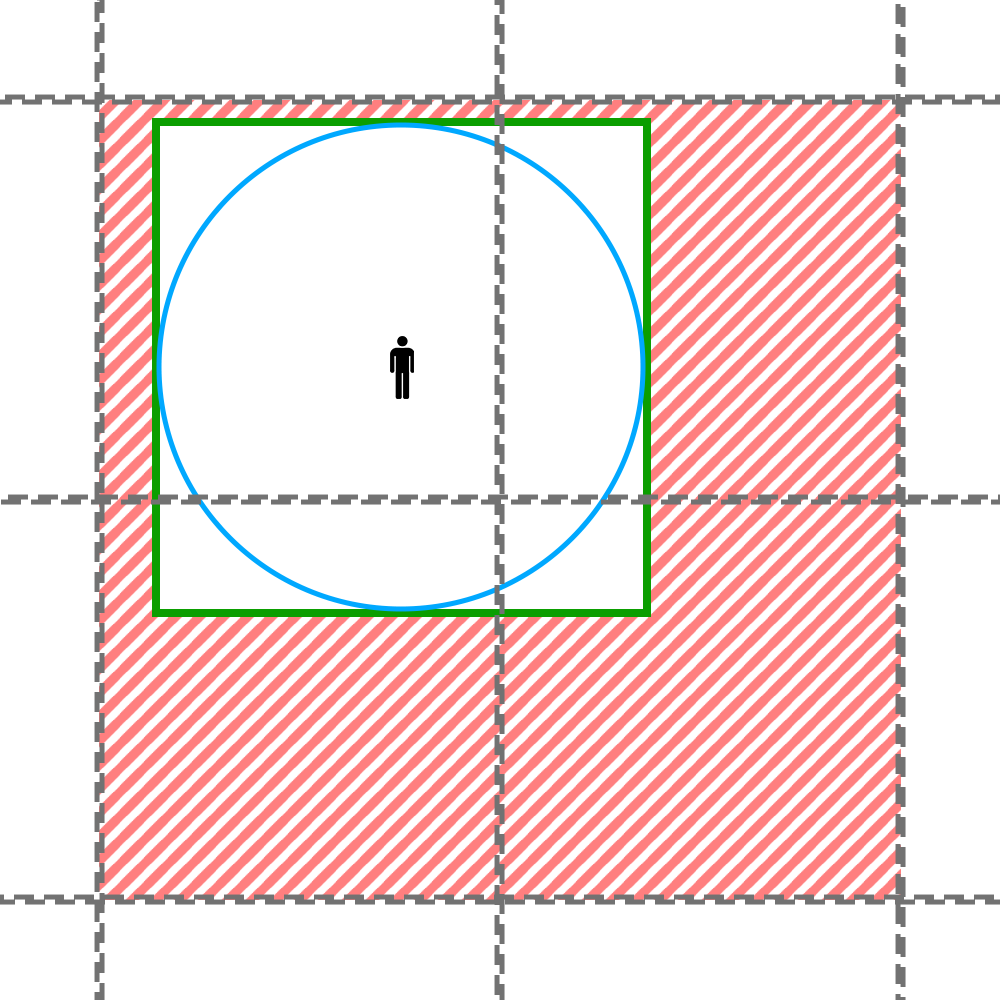
\includegraphics[width=0.5\linewidth]{img/odrzucenie_srtm.png}
    \caption{Wizualizacja usuwania niepotrzebnych danych SRTM.}
    \label{fig:drop-unused-data}
\end{figure}

Dzięki takiemu założeniu, ilość przetwarzanych danych została ograniczona nawet o $92,7\%$, jeśli maksymalna widoczność wynosi $30$km oraz brane są pod uwagę cztery sąsiadujące kratki. W przypadku gdy obserwator znajduje się w okolicach Tatr, to ze względu na zmniejszenie odległości między kolejnymi punktami długości geograficznej, różnica ta wynosi około $88,9\%$. Natomiast, jeśli maksymalny dystans jest ustawiony na $50$km, wartości te wynoszą odpowiednio $89,7\%$ i $79,2\%$.

Dane teoretyczne oraz wyniki pokazane w tabeli \ref{tab:render-drop-time-comp}, jednoznacznie potwierdzają zasadność takiego uproszczenia. Sumaryczny czas potrzebny na wygenerowanie modelu przy odrzuceniu części danych jest mniejszy o około $80-85\%$ w porównaniu do cyklu bez takiej optymalizacji.

\begin{table}[!h]
  \centering
  \caption{Porównanie czasu generowania wierzchołków i trójkątów przy uproszczeniu i braku uproszczenia danych.}
  \resizebox{\textwidth}{!}{%
  \begin{tabularx}{\linewidth}{|l|*{4}{>{\centering\arraybackslash}X|}}
    \hline
     Urządzenie & \begin{tabular}[c]{@{}c@{}}Czas \\ upraszczania \\ danych \end{tabular} & \begin{tabular}[c]{@{}c@{}}Czas \\ generowania\\ wierzchołków \end{tabular} & \begin{tabular}[c]{@{}c@{}}Czas \\ generowania\\ trójkątów \end{tabular}  & Sumaryczny czas\\
    \hline
    \hline
    \multicolumn{5}{|c|}{Bez upraszczania danych ($t_{1}$)} \\
    \hline
    Mate 20 Lite & nd. & 0,1730 s & 0,1255 s & 0,2985 s  \\
    \hline
    P30 Pro &  nd. & 0,0980 s & 0,1170 s & 0,0937 s \\
    \hline
    Mate 50 Pro &  nd. & 0,0549 s & 0,0586 & 0,1136 s \\
    \hline
    
    \multicolumn{5}{|c|}{Z upraszczaniem danych ($t_{2}$)} \\
    \hline
    Mate 20 Lite & 0,0033 s & 0,0387 s & 0,0227 s & 0,0648 s  \\
    \hline
    P30 Pro &  0,0016 s & 0,0142 s & 0,0154 s & 0,0314 s \\
    \hline
    Mate 50 Pro & 0,0007 s & 0,0081 s & 0,0079 s & 0,0168 s \\
    \hline
    
    \multicolumn{5}{|c|}{Stosunek czasów $\frac{t_{2}}{t_{1}}$} \\
    \hline

     Mate 20 Lite & nd. & 0,2241 & 0,1811 & 0,2171  \\
    \hline
    P30 Pro &  nd. & 0,1458 & 0,1651 & 0,1640 \\
    \hline
    Mate 50 Pro & nd. & 0,1478 & 0,1362 & 0,1458 \\
    \hline
    
  \end{tabularx}%
}
  \label{tab:render-drop-time-comp}
\end{table}





\subsection{Porównanie algorytmów obliczających odległość między dwoma punktami geograficznymi}

Ze względu na różne rozwiązania umożliwiające obliczenie odległości między dwoma punktami, zostały one przetestowane pod kątem dokładności wykonywanych obliczeń oraz szybkości działania.

Jako referencja wyników odległości wykorzystany został algorytm Vincenta, uznawany za najbardziej dokładny wśród prezentowanych. Ustawiony został dla niego limit iteracji na poziomie $1000$ (w nagłówkach tabel, liczba w nawiasie przy metodzie Vincenta oznacza maksymalną liczbę iteracji) i względem niego obliczane były różnice i błędy pozostałych metod.


Niezależnie od odległości wszystkie algorytmy uzyskały akceptowalną niedokładność wyników. Przedstawione zostały one w tabeli \ref{tab:geo-distance-accuracy}. Największa różnica wyniosła około $0,32\%$ dla przypadku Londyn - Warszawa, którego rzeczywista odległość wynosi $\sim1452$~km. Wartość ta odpowiada w przybliżeniu błędowi $200$ m. Na potrzeby obliczeń wykonywanych w ramach projektu dyplomowego, błąd przy tak odległych punktach jest całkowicie pomijalny i nie wpływa w istotny sposób na działanie programu i dokładność rezultatów całego procesu. Dodatkowo, obliczenia na tak dużych odległościach w projekcie są mało prawdopodobne, ponieważ widoczność tak oddalonych szczytów jest niemożliwa i w rzeczywistości nie występuje. Największe dystanse w aplikacji testowej obliczane są między dwoma bokami siatki geograficznej, ale nawet wtedy ich maksymalny wynik nie przekracza $220$ km. Jest to mniej niż badana wartość dla przypadku Warszawa - Kraków, dla którego błąd wynosi około $0,07\%$. 

\begin{table}[!h]  \centering
\caption{Porównanie dokładności wybranych algorytmów obliczających odległość między dwoma punktami geograficznymi.}
\resizebox{\textwidth}{!}{%
\begin{tabular} {| c | c | c | c | c | c |} \hline
\textbf{Punkty geograficzne} &
  \textbf{Vincent (1000)} &
  \textbf{Vincent (100)} &
  \textbf{Haversian} &
  \textbf{\begin{tabular}[c]{@{}c@{}}Spherical \\ Law of Cosines\end{tabular}} &
  \textbf{\begin{tabular}[c]{@{}c@{}}Equirectangular \\ Approximation\end{tabular}} \\
\hline \hline
(49.0; 20.0) -\textgreater (50.0; 20.0) &
  111,21941 km &
  \begin{tabular}[c]{@{}c@{}}111,21941 km\\ $\Delta=0,00000$ km\\ (0,00000\%)\end{tabular} &
  \begin{tabular}[c]{@{}c@{}}111,19493 km\\ $\Delta=0,02448$ km\\ (0,02201\%)\end{tabular} &
  \begin{tabular}[c]{@{}c@{}}111,19497 km\\ $\Delta=0,02444$ km\\ (0,02197\%)\end{tabular} &
  \begin{tabular}[c]{@{}c@{}}111,19493 km\\ $\Delta=0,02448$ km\\ (0,02201\%)\end{tabular} \\
\hline

(49.0; 20.0) -\textgreater (49.0; 21.0) &
  73,17126 km &
  \begin{tabular}[c]{@{}c@{}}73,17126 km\\ $\Delta=0,00000$ km\\ (0,00000\%)\end{tabular} &
  \begin{tabular}[c]{@{}c@{}}72,94991 km\\ $\Delta=0,22135$ km\\ (0,30251\%)\end{tabular} &
  \begin{tabular}[c]{@{}c@{}}72,94991 km\\ $\Delta=0,22135$ km\\ (0,30251\%)\end{tabular} &
  \begin{tabular}[c]{@{}c@{}}72,95044 km\\ $\Delta=0,22082$ km\\ (0,30179\%)\end{tabular} \\
\hline

\begin{tabular}[c]{@{}l@{}}(51.509865; -0.118092)\\ -\textgreater (52.237049; 21.017532)\\ Londyn -\textgreater Warszawa\end{tabular} &
  1452,71785 km &
  \begin{tabular}[c]{@{}c@{}}1452,71104 km\\ $\Delta=0,00681$ km\\ (0,00047\%)\end{tabular} &
  \begin{tabular}[c]{@{}c@{}}1448,08846 km\\ $\Delta=4,62939$ km\\ (0,31867\%)\end{tabular} &
  \begin{tabular}[c]{@{}c@{}}1448,08846 km\\ $\Delta=4,62939$ km\\ (0,31867\%)\end{tabular} &
  \begin{tabular}[c]{@{}c@{}}1453,24964 km\\ $\Delta=0,53179$ km\\ (0,03661\%)\end{tabular} \\
\hline

\begin{tabular}[c]{@{}l@{}}(52.237049; 21.017532)\\ -\textgreater (50.049683; 19.944544)\\ Warszawa -\textgreater Kraków\end{tabular} &
  254,66051  km &
  \begin{tabular}[c]{@{}c@{}}254,66057 km\\ $\Delta=0,00006$ km\\ (0,00002\%)\end{tabular} &
  \begin{tabular}[c]{@{}c@{}}254,74374 km\\ $\Delta=0,18677$ km\\ (0,07334\%)\end{tabular} &
  \begin{tabular}[c]{@{}c@{}}254,47374 km\\ $\Delta=0,18677$ km\\ (0,07334\%)\end{tabular} &
  \begin{tabular}[c]{@{}c@{}}254,48145 km\\ $\Delta=0,17906$ km\\ (0,07031\%)\end{tabular} \\
\hline

\begin{tabular}[c]{@{}l@{}}(50.049683; 19.944544)\\ -\textgreater (49.299030; 19.949047)\\ Kraków -\textgreater Zakopane\end{tabular} &
  83,49035 km &
  \begin{tabular}[c]{@{}c@{}}83,49035 km\\ $\Delta=0,00000$ km\\ (0,00000\%)\end{tabular} &
  \begin{tabular}[c]{@{}c@{}}83,46943 km\\ $\Delta=0,02092$ km\\ (0,02506\%)\end{tabular} &
  \begin{tabular}[c]{@{}c@{}}83,46943 km\\ $\Delta=0,02092$ km\\ (0,02506\%)\end{tabular} &
  \begin{tabular}[c]{@{}c@{}}83,46943 km\\ $\Delta=0,02092$ km\\ (0,02506\%)\end{tabular} \\
\hline

\begin{tabular}[c]{@{}l@{}}(49.299030; 19.949047)\\ -\textgreater (49.250332; 19;933662)\\ Zakopane -\textgreater Giewont\end{tabular} &
  5,53040 km &
  \begin{tabular}[c]{@{}c@{}}5,53040 km\\ $\Delta=0,00000$ km\\ (0,00000\%)\end{tabular} &
  \begin{tabular}[c]{@{}c@{}}5,52875 km\\ $\Delta=0,00165$ km\\ (0,02984\%)\end{tabular} &
  \begin{tabular}[c]{@{}c@{}}5,52875 km\\ $\Delta=0,00165$ km\\ (0,02984\%)\end{tabular} &
  \begin{tabular}[c]{@{}c@{}}5,52875 km\\ $\Delta=0,00165$ km\\ (0,02984\%)\end{tabular}  \\
\hline

\end{tabular}%
}
\label{tab:geo-distance-accuracy}
\end{table}


W przypadku obliczania odległości między dwoma równoleżnikami błąd porównywanych algorytmów wynosił około $0,022\%$. Natomiast niedokładność wyników między południkami był na poziomie $0,30\%$. Te dwa testy ze względu na swoje znaczenie przy wyznaczaniu skali generowanego modelu trójwymiarowego, która ma realny wpływ na dokładność rozpoznawania szczytów, były bardzo istotne. Pomijając algorytm Vincenta, pozostałe metody dały porównywalne wyniki. Z tego powodu ich wpływ na wybór ostatecznej metody był zerowy. Tym bardziej, że przekłamanie w obliczonym dystansie wynosiło odpowiednio tylko $20$ m i $200$ m.

\par

Algorytm Vincenta, niezależnie od wartości parametru maksymalnej liczby iteracji daje praktycznie takie same rezultaty. Może to wynikać z charakterystyki tej metody oraz wykorzystanych danych wejściowych w trakcie testu. Prawdopodobnie w badanych przypadkach algorytm przestawał obliczać kolejne przybliżenia wartości przed osiągnięciem zadanej, maksymalnej liczby iteracji. Mogło to wynikać z faktu osiągnięcia błędu mniejszego niż $\varepsilon=1\mathrm{e}{-12}$.

\par

Niedokładność podczas obliczania odległości między Krakowem, a Zakopanem wyniosła w przybliżeniu $20$ m. Jest to wartość mniejsza niż odległość między kolejnymi punktami danych \textit{SRTM1}, których rozdzielczość wynosi około $30$ m. Błąd na tym poziomie uzyskały wszystkie testowane metody. Z tego powodu ostateczny wybór algorytmu jako optymalny z zaprezentowanych odbywał się z uwzględnieniem przede wszystkim złożoności czasowej poszczególnych rozwiązań.

Takie porównanie czasu trwania obliczeń dla poszczególnych rozwiązań przedstawiono w tabeli \ref{tab:geo-distance-time}. Zgodnie z założeniami, w porównaniu do metody Vincenta trzy pozostałe algorytmy okazały się dużo szybsze.

\begin{table}[!h]  \centering\hfill
\caption{Porównanie czasu wykonania wybranych algorytmów obliczających odległość między dwoma punktami geograficznymi.}
\resizebox{\textwidth}{!}{%
\begin{tabular} {| c | c | c | c | c | c | c |} \hline
    Urządzenie &
   &
  \textbf{Vincent (1000)} &
  \textbf{Vincent (100)} &
  \textbf{Haversian} &
  \textbf{\begin{tabular}[c]{@{}l@{}}Spherical\\ Law of Cosines\end{tabular}} &
  \textbf{\begin{tabular}[c]{@{}l@{}}Equirectangular\\ Approximation\end{tabular}} \\
  \hline \hline
  
  
\multicolumn{1}{|l|}{\multirow{3}{*}{\begin{tabular}[c]{@{}l@{}}\hphantom{abc}\\  \\ \\ Mate 20 Lite\end{tabular}}} &
  \multicolumn{1}{l|}{\begin{tabular}[c]{@{}l@{}}Średni czas\\ jednego testu\end{tabular}} &
  \multicolumn{1}{l|}{10,97529 s} &
  \multicolumn{1}{l|}{11,52881 s} &
  \multicolumn{1}{l|}{2,25107 s} &
  \multicolumn{1}{l|}{2,06024 s} &
  \multicolumn{1}{l|}{0,59029 s} \\ \cline{2-7} 
\multicolumn{1}{|l|}{} &
  \multicolumn{1}{l|}{\begin{tabular}[c]{@{}l@{}}Średni czas\\ wywołania\\ jednej funkcji\end{tabular}} &
  \multicolumn{1}{l|}{1097,52893 ns} &
  \multicolumn{1}{l|}{1152,88094 ns} &
  \multicolumn{1}{l|}{225,10736 ns} &
  \multicolumn{1}{l|}{206,02364 ns} &
  \multicolumn{1}{l|}{59,02929 ns} \\ \cline{2-7} 
\multicolumn{1}{|l|}{} &
  \multicolumn{1}{l|}{\begin{tabular}[c]{@{}l@{}}Różnica czasowa\\ jednego wywołania\\ funkcji\end{tabular}} &
  \multicolumn{1}{l|}{nd.} &
  \multicolumn{1}{l|}{\begin{tabular}[c]{@{}l@{}}-55,35201 ns\\ (-4,80119\%)\end{tabular}} &
  \multicolumn{1}{l|}{\begin{tabular}[c]{@{}l@{}}-927,77358 ns\\ (-80,47436\%)\end{tabular}} &
  \multicolumn{1}{l|}{\begin{tabular}[c]{@{}l@{}}-946,85730 ns\\ (-82,12967\%)\end{tabular}} &
  \multicolumn{1}{l|}{\begin{tabular}[c]{@{}l@{}}-1093,85165 ns\\ (-94,87982\%)\end{tabular}} \\
  \hline
  
  
\multicolumn{1}{|l|}{\multirow{3}{*}{\begin{tabular}[c]{@{}l@{}}\hphantom{abc}\\  \\ \\ P30 Pro\end{tabular}}} &
  \multicolumn{1}{l|}{\begin{tabular}[c]{@{}l@{}}Średni czas\\ jednego testu\end{tabular}} &
  \multicolumn{1}{l|}{4,84974 s} &
  \multicolumn{1}{l|}{4,83854 s} &
  \multicolumn{1}{l|}{0,89253 s} &
  \multicolumn{1}{l|}{0,91203 s} &
  \multicolumn{1}{l|}{0,35220 s} \\ \cline{2-7} 
\multicolumn{1}{|l|}{} &
  \multicolumn{1}{l|}{\begin{tabular}[c]{@{}l@{}}Średni czas\\ wywołania \\ jednej funkcji\end{tabular}} &
  \multicolumn{1}{l|}{484,97448 ns} &
  \multicolumn{1}{l|}{483,85403 ns} &
  \multicolumn{1}{l|}{89,25293 ns} &
  \multicolumn{1}{l|}{91,20310 ns} &
  \multicolumn{1}{l|}{35,22035 ns} \\ \cline{2-7} 
\multicolumn{1}{|l|}{} &
  \multicolumn{1}{l|}{\begin{tabular}[c]{@{}l@{}}Różnica czasowa\\ jednego wywołania\\ funkcji\end{tabular}} &
  \multicolumn{1}{l|}{nd.} &
  \multicolumn{1}{l|}{\begin{tabular}[c]{@{}l@{}}+1,12045 ns\\ (+0,23157 \%)\end{tabular}} &
  \multicolumn{1}{l|}{\begin{tabular}[c]{@{}l@{}}-394,60110 ns\\ (-81,55375\%)\end{tabular}} &
  \multicolumn{1}{l|}{\begin{tabular}[c]{@{}l@{}}-392,65093 ns\\ (-81,15070\%)\end{tabular}} &
  \multicolumn{1}{l|}{\begin{tabular}[c]{@{}l@{}}-448,63368 ns\\ (-92,72087\%)\end{tabular}} \\
  \hline
  
  
\multicolumn{1}{|l|}{\multirow{3}{*}{\begin{tabular}[c]{@{}l@{}}\hphantom{abc}\\  \\ \\ Mate 50 Pro\end{tabular}}} &
  \multicolumn{1}{l|}{\begin{tabular}[c]{@{}l@{}}Średni czas\\ jednego testu\end{tabular}} &
  \multicolumn{1}{l|}{3,98607 s} &
  \multicolumn{1}{l|}{3,92896 s} &
  \multicolumn{1}{l|}{0,66648 s} &
  \multicolumn{1}{l|}{0,60028 s} &
  \multicolumn{1}{l|}{0,15715 s} \\ \cline{2-7} 
\multicolumn{1}{|l|}{} &
  \multicolumn{1}{l|}{\begin{tabular}[c]{@{}l@{}}Średni czas\\ wywołania\\ jednej funkcji\end{tabular}} &
  \multicolumn{1}{l|}{398,60748 ns} &
  \multicolumn{1}{l|}{392,8963 ns} &
  \multicolumn{1}{l|}{66,64805 ns} &
  \multicolumn{1}{l|}{60,02849 ns} &
  \multicolumn{1}{l|}{15,71475 ns} \\ \cline{2-7} 
\multicolumn{1}{|l|}{} &
  \multicolumn{1}{l|}{\begin{tabular}[c]{@{}l@{}}Różnica czasowa\\ jednego wywołania\\ funkcji\end{tabular}} &
  \multicolumn{1}{l|}{nd.} &
  \multicolumn{1}{l|}{\begin{tabular}[c]{@{}l@{}}+5,71118 ns\\ (+1,45361\%)\end{tabular}} &
  \multicolumn{1}{l|}{\begin{tabular}[c]{@{}l@{}}-326,24825 ns\\ (-83,03673\%)\end{tabular}} &
  \multicolumn{1}{l|}{\begin{tabular}[c]{@{}l@{}}-332,86781 ns\\ (-84,72154\%)\end{tabular}} &
  \multicolumn{1}{l|}{\begin{tabular}[c]{@{}l@{}}-377,18155 ns\\ (-96,00028\%)\end{tabular}} \\
  \hline


\end{tabular}%
}
\label{tab:geo-distance-time}
\end{table}




Przy badaniu złożoności obliczeniowej algorytmu Vincenta dla obu wartości parametrów czas wykonania funkcji i testu był podobny. Wynik ten wydaje się potwierdzać tezę, że maksymalna liczba iteracji nie jest osiągana, a proces kończy działanie wcześniej. 

\par

Metody Haverisan oraz Sferyczne Prawo Consinusów opierają się na bardzo podobnej metodzie i obliczeniach, dlatego czas ich wykonania jest bardzo zbliżony. Obliczenie jednego wywołania tych dwóch funkcji zajmuje jedynie około $20\%$ czasu potrzebnego na wykonanie algorytmu Vincenta. W przypadku najsłabszego z wykorzystanych urządzeń jest to różnica prawie tysiąc nanosekund przy każdej obliczanej odległości.

\par

Najszybszym z testowanych sposobów obliczenia odległości między dwoma punktami geograficznymi jest przybliżenie Equirectangular. Nawet względem najbardziej popularnej formuły Haversiana wykonywany jest $3-4$ razy szybciej. Jest to zgodne z przedstawionym teoretycznym opisem teoretycznym tej metody, gdzie stwierdzono jej popularność przy projektach o ograniczonych zasobach sprzętowych ze względu na jej małą złożoność obliczeniową.



Na podstawie przyprowadzonych testów dokładności i szybkości działania na urządzeniach testowych wybrany jako najbardziej optymalny został algorytm Equirectangular Approximation. Uzyskał on podobny błąd odległości jak pozostałe metody, ale jego złożoność czasowa była znacznie mniejsza. Szybkość działania była czynnikiem decydującym ze względu na złożoność czasową, co w przypadku urządzeń mobilnych, których zasoby są ograniczone może mieć bardzo istotne znaczenie. 



\subsection{Testowanie i optymalizacja algorytmów dopasowania obrazów} \label{sec:test_matching}

Dopasowanie obrazów celem stwierdzenia widoczności wybranych gór oraz określenia ich położenia na zdjęciu wydaje się zagadnieniem kluczowym w kontekście prawidłowego rozpoznawania szczytów. Z tego powodu przeprowadzone zostały testy porównujące algorytmy oparte na szablonach oraz na cechach. Przebadano została także ich skuteczność w~zależności od ustawień wybranych parametrów. Odbywało się to poprzez przeszukanie przestrzeni możliwych ich wartości celem znalezienia najbardziej optymalnych zestawień. Przeprowadzono również badanie sprawdzające jaki wpływ ma operacja morfologiczna dylacji na jakość klasyfikatorów przy zastosowaniu jej na obrazach binarnych. Wykonane badania pozwoliły na wybranie lepszej metody, dobranie parametrów optymalnych oraz stwierdzenie czy wykorzystanie dylacji jest uzasadnione.

Opisane w poniższych podrozdziałach testy zostały przeprowadzone z wykorzystaniem dwóch zdjęć ze zbioru przygotowanego do statycznej analizy podczas jednego z etapów pracy dyplomowej. Na obu z nich widoczne są inne szczyty, jednak wszystkie należą do pasma górskiego Tatr. Na potrzeby testów, badane zdjęcia zostały kilkukrotnie powielone i~zmodyfikowane poprzez dodanie na kolejnych kopiach różnego typu artefaktów. Zmiany te miały symulować niewidoczność szczytów górskich, które mogą wystąpić z różnych względów w rzeczywistości. Takimi powodami mogą być na przykład przesłanianie innymi obiektami, drzewami czy budynkami. Dwie z takich takich modyfikacji pokazane zostały na rysunku \ref{fig:not_visible_peaks}. Każde zdjęcie występuje w sumie w sześciu wariantach, na których zasłaniane są pojedyncze szczyty, kilka na raz lub całe pasma, większymi lub mniejszymi elementami. 

\begin{figure}[!h]
    \centering 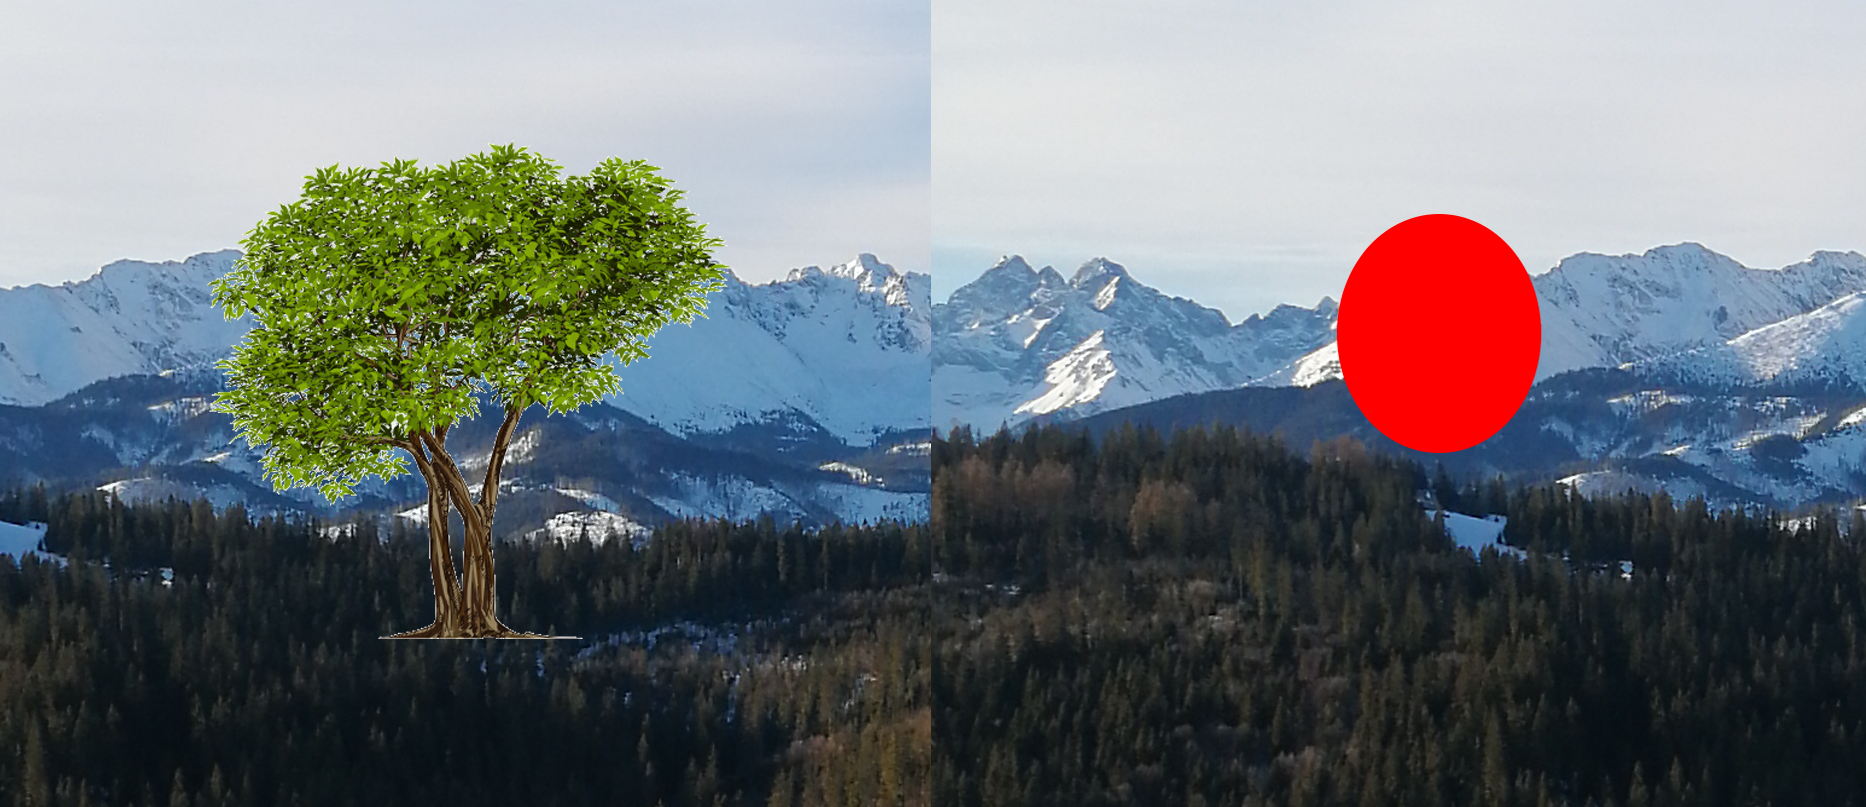
\includegraphics[width=.9\linewidth]{img/zaslanianie_przyklad.png}
    \caption{Przykłady nałożenia artefaktów zasłaniających część szczytów w wybranych przypadkach testowych.}
    \label{fig:not_visible_peaks}
\end{figure}

Sumarycznie daje to $378$ badanych szczytów w pojedynczym teście (każda kopia jednego zdjęcia - $32$ szczyty, natomiast drugiego - $31$), w tym $199$ widocznych oraz $179$ zasłoniętych. Daje to rozkład klas na poziomie $53\%/47\%$.

Badania były przeprowadzane przy dwóch rozdzielczościach: $768\textrm{x}1024$ i $3840\textrm{x}5120$. Większa z nich związana jest z wielkością zebranych wcześniej statycznych zdjęć. Model trójwymiarowy terenu był domyślnie generowany w rozmiarach $768\textrm{x}1024$, dlatego w przypadku drugiej rozdzielczości zdjęć, uzyskany render interpolowany był w górę. Operacja ta była przeprowadzana dopiero na wynikowym obrazie binarnym procesu detekcji krawędzi.

W poniższych zestawieniach i porównaniach przedstawione zostały wyniki jedynie dla mniejszego rozmiaru zdjęć, ponieważ w procesie rozpoznawania szczytów w czasie rzeczywistym wykorzystywane są obrazy o mniejszych rozdzielczościach ze względu na złożoność czasową obliczeń. Dlatego rozmiar $768\textrm{x}1024$ jest bliższy rzeczywistemu. Dodatkowo, przestrzeń w pracy dyplomowej zajmowana przez tak dużą ilość danych rozrosłaby się niepotrzebnie. Porównanie dwóch rozdzielczości pozwoliło jednak stwierdzić brak znaczących różnic w wynikach między nimi. Z tego względu można założyć, że wpływ rozdzielczości zdjęć na skuteczność dopasowania obrazów do siebie nie jest tak znaczny. Wszelkie dane zebrane dla obu rozdzielczości zostały umieszczone w repozytorium opisanym w załączniku nr 1. 


W zależności od rozmiaru zdjęcia badane były różne rozmiary wycinka obrazów. W~przypadku rozdzielczości $768\textrm{x}1024$ były to fragmenty o wymiarach: $20\textrm{x}20$, $40\textrm{x}40$, $60\textrm{x}60$, $80\textrm{x}80$, $120\textrm{x}120$, $160\textrm{x}160$, $200\textrm{x}200$, $300\textrm{x}300$. Natomiast, dla $3840\textrm{x}5120$: $100\textrm{x}100$, $200\textrm{x}200$, $300\textrm{x}300$, $400\textrm{x}400$, $600\textrm{x}600$, $800\textrm{x}800$, $1000\textrm{x}1000$. Wycinany segment zdjęcia rzeczywistego był powiększony o $15\%$ rozmiaru zdjęcia. Związane jest to z założoną niedokładnością czujników dotyczących obrotu urządzenia. Założona tolerancja odpowiada około $+/-5^\circ$ odchylenia w każdym kierunku. Sprawia to, że wycinki zdjęć mają rozmiary odpowiednio $\{250\textrm{x}328$, $270\textrm{x}348$, $190\textrm{x}368$, $310\textrm{x}388$, $350\textrm{x}428$, $390\textrm{x}68$, $430\textrm{x}508$, $530\textrm{x}608\}$ (powiększenie o $230\textrm{x}308$) i $\{1252\textrm{x}1636$, $1352\textrm{x}1736$, $1452\textrm{x}1836$, $1552\textrm{x}1936$, $1752\textrm{x}2136$, $1952\textrm{x}2336$, $2152\textrm{x}2536\}$ (powiększenie $576\textrm{x}768$).

W przypadku dopasowania opartego na szablonach, badano wszystkie rozmiary wycinków, zarówno dla korelacji krzyżowej, jaki i współczynnika korelacji krzyżowej. Dla każdego wyniku klasyfikatora wybierana była jedynie najwyższa wartość prawdopodobieństwa uznawana za hipotetyczne położenie szczytu. Pozostałe rezultaty były odrzucane. Najpierw jednak, dla każdego ustawienia algorytmu ustalana była wartość progu. Odbywało się to poprzez wyliczenie dla każdej kombinacji współczynników wszystkich przypadków testowych. Na ich podstawie dobierana była taka wartość, przy której liczba poprawnych wskazań była największa. Przykład wartości wykorzystanych do wyznaczenia progu pokazano na rysunku \ref{fig:template_threshold}. Wykres ten przedstawia uzyskane wartości prawdopodobieństwa dopasowania podzielone na trzy grupy: prawidłowo określone położenie, błędnie określone położenie oraz szczyt niewidoczny na zdjęciu rzeczywistym. Na rysunku została zaznaczona również wartość progu wybrana dla tego ustawienia algorytmu. Przy tak wyliczonych limitach przeprowadzano dalsze testy dla tej metody. 

\begin{figure}[!h]
    \centering 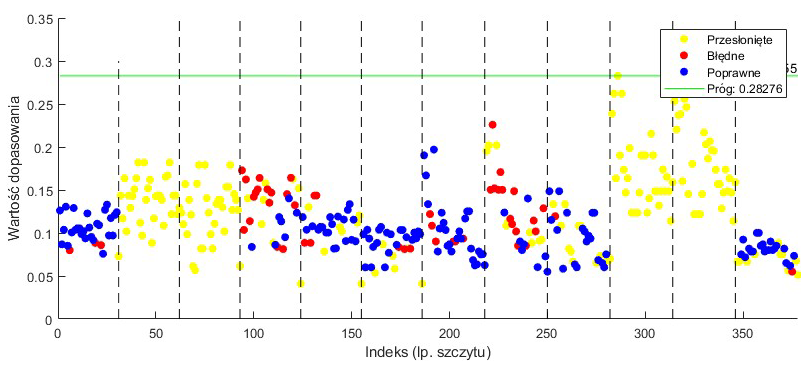
\includegraphics[width=1\linewidth]{img/przyklad_threshold.png}
    \caption{Przykład obliczonego podobieństwa dla poszczególnych przypadków przy użyciu algorytmu dopasowania szablonu. Na ich podstawie ustalany był próg wartości dla danych ustawień parametrów.}
    \label{fig:template_threshold}
\end{figure}

Feature matching zostało podzielone na cztery kategorie testów, po dwie dla każdego rodzaju dopasowania. Zarówno dla metody opartej na metodzie siłowej, jak i FLANN, były to progowanie punktów kluczowych i przeprowadzenie testu współczynników dla k-najbliższych sąsiadów. Każda z nich była badana dla  deskryptorów i cech charakterystycznych uzyskanych przy pomocy algorytmów SIFT i ORB. W przypadku filtracji więcej niż jednej pary przy pomocą testu ratio, badane były następujące wartości tego parametru: $\{0,9$, $0,75$, $0,6$, $0,5\}$. Natomiast, gdy wykorzystywane było progowanie najpierw ustalone zostały wartości graniczne dla poszczególnych przypadków testowych. Odbywało się to na podobnej zasadzie co w przypadku dopasowania na podstawie szablonu. Ze względu jednak, że dla metody opartej na cechach, liczba wartości obliczana na jeden szczyt jest większa niż w przypadku template matching, to określone zostały trzy wartości progów dla każdego ustawienia. Oznaczały one branie pod uwagę różnej liczby najlepszych trafień.  W obu filtracjach i dla każdego algorytmu wykrywania cech, badano również maksymalną liczbę dopasowań braną pod uwagę przy procesie projekcji homograficznej: bez ograniczeń, $10$ lub $20$. 

W poszczególnych przypadkach testowych, dla każdego szczytu przypisywany jest jeden z czterech możliwych wyników:

\begin{itemize}
    \item \textbf{TP} (ang. True Positive) - prawdziwie pozytywne. Przypadki, które zostały poprawnie sklasyfikowane jako pozytywne - szczyt został poprawnie uznany za widoczny na zdjęciu, a jego położenie mieści się w granicach przyjętego błędu.
    \item \textbf{TN} (ang. True Negative) - prawdziwie negatywne. Przypadki, które zostały poprawnie sklasyfikowane jako negatywne - szczyt został poprawnie uznany za niewidoczny na zdjęciu.
    \item \textbf{FP} (ang. False Positive) - fałszywie pozytywne. Przypadki, które zostały błędnie sklasyfikowane jako pozytywne - szczyt został niepoprawnie uznany za widoczny lub jego estymowane położenie jest zbyt odległe od prawidłowego. 
    \item \textbf{FN} (ang. False Negative) - fałszywie negatywne. Przypadki, które zostały błędnie sklasyfikowane jako negatywne - szczyt został błędnie uznany jako niewidoczny.
\end{itemize}

Na ich podstawie obliczane były cztery wskaźniki skuteczności klasyfikatora: dokładność, precyzja, czułość i miara F1 \cite{metrics}. W ogólności dla każdego z nich im większa wartość tym lepiej. Jednak dla lepszej interpretacji wyników wymagana jest analiza wszystkich wskaźników oraz liczby przypadków sklasyfikowanych jako TP, TN, FP i FN.

\paragraph{Dokładność.} Stosunek poprawnie sklasyfikowanych przypadków do sumy wszystkich testów. Określa ogólną skuteczność klasyfikatora.
\begin{align*}
\textrm{Dokładność} =  \frac{TP + TN}{TP+TN+FP+FN}
\end{align*} 


\paragraph{Precyzja.} Liczba poprawnie pozytywnych przypadków do sumy prawdziwie i fałszywie pozytywnych wyników. Opisuje ile pozytywnych przypadków jest faktycznie prawdziwych. 
\begin{align*}
\textrm{Precyzja} = \frac{TP}{TP+FP}
\end{align*} 


\paragraph{Czułość.} Proporcja prawdziwie pozytywnych rezultatów do sumy poprawnych pozytywów i fałszywych negatywów. Wyraża zdolność do wykrywania pozytywnych przypadków.
\begin{align*}
\textrm{Czułość} =  \frac{TP}{TP+FN}
\end{align*} 

\paragraph{Miara F1.} Jest to średnia harmoniczna precyzji i czułości. Pozwala określić jednym wskaźnikiem skuteczność klasyfikatora biorąc pod uwagę te dwie składowe. 
\begin{align*}
\textrm{F1} =  \frac{2*\textrm{Precyzja}*\textrm{Czułość}}{\textrm{Precyzja}+\textrm{Czułość}}
\end{align*} 


Estymowane położenie szczytu na obrazie było uznawane za poprawne, jeśli spełniało nierówność związaną z odległością od oczekiwanego rezultatu:

\begin{align*}
    \lVert \text{P} - \text{E} \rVert \le K*\sqrt{w^2 + h^2}
\end{align*}

gdzie: 
 
\begin{itemize}
    \item \textbf{P} (ang. Predicted) - obliczone położenie szczytu na obrazie.
    \item \textbf{E} (ang. Expected) - oczekiwane (prawidłowe) położenie szczytu na obrazie.
    \item \textbf{K} - współczynnik skalujący, określający dopuszczalną wielkość błędu.
    \item \textbf{w, h} - wymiary obrazu.
\end{itemize}


Współczynnik $K$ pozwala określić wielkość dopuszczalnego błędu zwróconego położenia względem oczekiwanego. Oznacza on to jak dokładna predykcja położenia szczytu na obrazie jest uznawana za wystarczającą. W trakcie testów wykorzystywane były wartości tego współczynnika równe $0,05$ i $0,01$. Dla rozmiaru zdjęcia $768\textrm{x}1024$ oznaczało to dopuszczalną odległość o wielkościach odpowiednio $64$ i $12,8$ pikseli. Interpretacja graficzna opisanych wartości współczynnika została pokazana na rysunku \ref{fig:wspolczynnik_K}. Przedstawia on przestrzeń, w której musi znajdować się wyliczone położenie szczytu by wynik został uznany za prawidłowy. Zewnętrzny obszar przedstawia wartość $K=0,05$, natomiast wewnętrzny $K=0,01$. Punkt oznaczony kropką oznacza idealne dopasowanie. Wybrany do tej prezentacji szczyt oddalony jest od obserwatora o około $13$ km. W tym przypadku wskazania na obwodzie szerszego okręgu wydają się zbyt odstające od rzeczywistego położenia by można uznać je za dokładne. Przy bliższych szczytach niedokładność nie byłaby tak wyraźna. Jednak z powodu, że w hipotetycznych warunkach rzeczywistych bardziej wartościowe wydają się wskazania dla gór będących w pewnej odległości od obserwatora, przy ostatecznym wyborze algorytmu większą uwagę zwracano na wyniki dla $K=0,01$.

\begin{figure}[!h]
    \centering 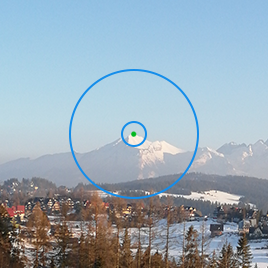
\includegraphics[width=0.4\linewidth]{tex/sections/wspolczynnik_K.png}
    \caption{Dopuszczalny błąd dopasowania w zależności od wartości współczynnika tolerancji~$K$ dla wybranego szczytu.}
    \label{fig:wspolczynnik_K}
\end{figure}


\subsubsection{Wpływ dylacji na skuteczność dopasowania obrazów} \label{sec:test_dilation}

Dylacja \cite{dilation} - jedna z operacji morfologicznych stosowanych w przetwarzaniu cyfrowym obrazu. Służy do zwiększania oraz łączenia obiektów, wypełniania dziur czy pogrubienia konturów i linii. Polega na modyfikacji każdego piksela w zależności od jego sąsiedztwa określonego rozmiarem elementu strukturalnego (najczęściej macierzy kwadratowej) będącej parametrem dylacji. Jeśli badany punkt ma w okolicy przynajmniej jeden piksel o wartości $255$ (lub $1,0$ w zależności od sposobu reprezentacji koloru białego) to przyjmuje on również tę wartość. 

Operacja dylacji może być również przeprowadzona z wykorzystaniem funkcji zwracającej wartość maksymalną z danego zbioru. W tym wypadku ze wszystkich wartości pikseli będących w danym sąsiedztwie. Wtedy wzór na tę operację morfologiczną można zapisać jako:

\begin{align*}
     (I \oplus B)(x, y) = \max \left\{ I(x + b, y + c) : (b, c) \in B \right\}
\end{align*}

gdzie $\textbf{I(x,y)}$ oznacza wartość danego piksela (luminancję), natomiast $\textbf{B}$ element strukturalny.

Podczas generowania grafik związanych z dopasowaniem obrazów na potrzeby pracy magisterskiej, został wykorzystany mechanizm dylacji celem poprawy ich czytelności. W~trakcie tego procesu, dla wybranego szczytu zaobserwowana została poprawa wskazania jego lokalizacji oraz zwiększenie wartości prawdopodobieństwa prawidłowego dopasowania. Mając to na uwadze, przeprowadzono wstępne testy wpływu dylacji na działanie algorytmów porównujących podobieństwo zdjęć przy losowych ustawieniach algorytmów. 

Przedstawione na rysunku \ref{fig:dilation_graph} wykresy punktowe prezentują wartości dopasowania szablonów poszczególnych szczytów dla jednakowych ustawień algorytmu, przy niemodyfikowanym zdjęciu oraz przy użytej dylacji. 

\begin{figure}[!h]
    \centering 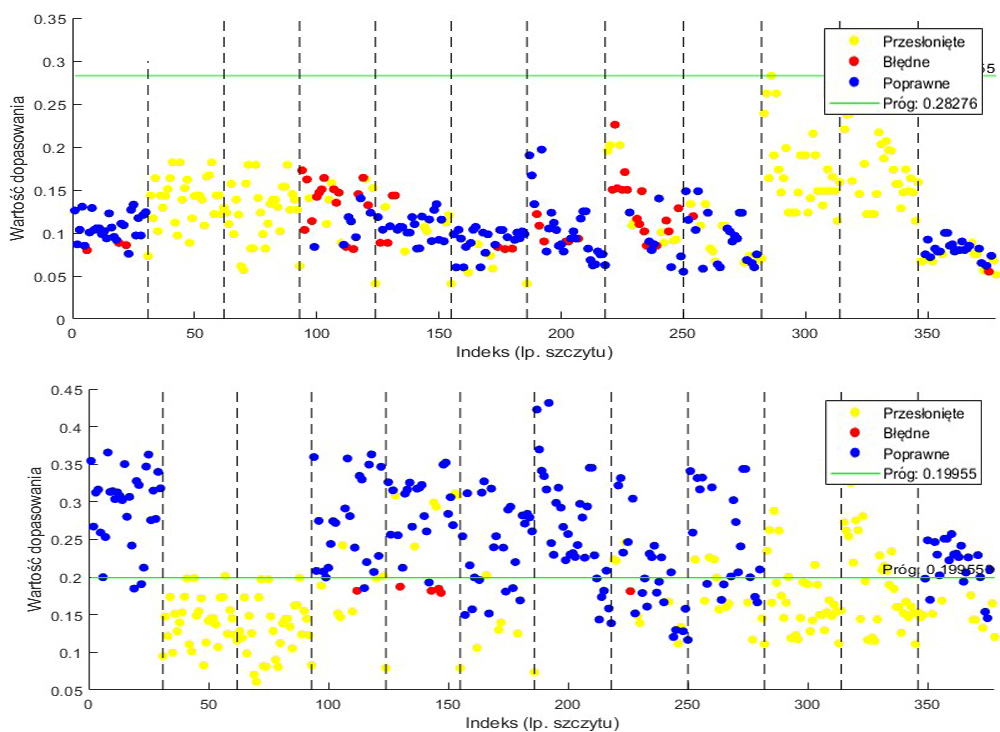
\includegraphics[width=0.93\linewidth]{img/dilation_graph.png}
    \caption{Przykład wpływu dylacji na wyniki algorytmu dopasowania obrazów na podstawie szablonów przy przykładowych ustawieniach parametrów. Górny wykres przedstawia wyniki bez wykorzystania dylacji, dolny natomiast z wykorzystaniem dylacji.}
    \label{fig:dilation_graph}
\end{figure}

Wskazania dla szczytów poprawnie oraz błędnie sklasyfikowanych, a także przesłoniętych przyjmują podobny zakres wartości w przypadku obrazów niemodyfikowanych. Widoczne to jest na górnym wykresie. Ciężko jest na nim wskazać jakikolwiek trend zachowania algorytmu i dobrać sensowną wartość progowania. Najlepszą wartość dokładności klasyfikatora metoda uzyskuje przy progu, dla którego wszystkie testy oznaczone zostają jako negatywne. Takie ewentualne działanie klasyfikatora nie jest w żaden sposób porządne i sensowne. Natomiast na wykresie dolnym, który pokazuje wyniki gdy obrazy zostały poddane operacji dylacji, można zaobserwować zwiększenie liczby poprawnych detekcji. Przede wszystkim jednak widoczny jest na nim pewien trend związany z wartościami w zależności od widoczności szczytu. Dla gór, które na zdjęciu rzeczywistym są niewidoczne, algorytm zwraca wartości zauważalnie niższe niż w przypadku, gdy szczyt znajduje się na zdjęciu. Dzięki temu, możliwe jest dobranie wartości progowania w sposób bardziej racjonalny. W~tym przypadku, przekłada się to na zdecydowane zwiększenie dokładności klasyfikatora. 


W tabeli \ref{tab:dilation} pokazano porównanie przykładowych wyników dopasowania obrazów z wykorzystaniem dylacji i bez. Są to rezultaty dla algorytmów wykorzystujących porównanie wzorca oraz cech przy losowo wybranych ustawieniach ich parametrów. W obu przypadkach użycie operacji morfologicznej pozwoliło zwiększyć wartości wszystkich metryk. Dla feature matching w przypadku czułości i miary F1 wskazania poprawione zostały o około $20$ punktów procentowych. Udało mu się też sklasyfikować prawie czterokrotnie więcej przypadków jako prawdziwie pozytywne. Badane ustawienie template matching dużo bardziej widocznie poprawiło się po zastosowaniu operacji dylacji. Sprawiła ona, że klasyfikator nie wskazywał już wszystkich przypadków jako negatywne. Pozwoliło to określić aż 151 szczytów jako prawdziwie pozytywne, zwiększając dokładność o $30$~punktów procentowych. Ze względu na pierwotne wskazanie wszystkich przypadków jako negatywne, gdy algorytm nie wykorzystywał dylacji, pozostałe wskaźniki były wtedy równe $0\%$. Użycie operacji morfologicznej oznaczało skok wartości tych metryk do poziomu~$\sim80\%$. Jest to niebagatelna i znacząca poprawa jakości tego klasyfikatora.

\begin{table}[!h]
  \centering
  \small
  \caption{Porównanie skuteczności algorytmów dopasowania obrazów na podstawie szablonu oraz na podstawie cech przy przykładowych ustawieniach parametrów tych metod z wykorzystaniem operacji dylacji oraz bez.}
\resizebox{\textwidth}{!}{%
  \begin{tabularx}{\linewidth}{|l|*{8}{>{\centering\arraybackslash}X|}}
    \hline
     &
     \vspace{0.5em}TP & 
     \vspace{0.5em}TN  & 
     \vspace{0.5em}FP & 
     \vspace{0.5em}FN  & 
     \hspace{0em}\textbf{Dokładność}  &
     \vspace{0.01ex}\hspace{0em}\textbf{Precyzja}   & 
     \vspace{0.01ex}\hspace{0em}\textbf{Czułość} &
     \vspace{0.5em}\textbf{F1} \\
    \hline
    \hline
    \multicolumn{9}{|c|}{Dopasowanie na podstawie szablonu} \\
    \hline
    Bez dylacji  & 0 & 179 & 0 & 199 & $47,3\%$ & $0,00\%$ & $0,00\%$ & $0,00\%$ \\
    \hline
    Z dylacją &  151 & 145 & 34 & 48 & $78,3\%$ & $81,6\%$ & $75,8\%$ &  $78,6\%$ \\
    \hline
    
    \multicolumn{9}{|c|}{Dopasowanie na podstawie cech} \\
    \hline
    Bez dylacji  & 10 & 164 & 22 & 182 & $46,0\%$ & $31,2\%$ & $5,2\%$ & $8,9\%$  \\
    \hline
    Z dylacją & 39 & 144 & 71 & 124 & $48,4\%$ & $35,4\%$ & $23,9\%$ & $28,3\%$  \\
    \hline
    
  \end{tabularx}%
}
  \label{tab:dilation}
\end{table}



Wyżej wymienione przykłady poprawy jakości klasyfikatora dzięki użyciu operacji dylacji sugerują zasadność wykorzystania tej techniki dla procesu porównania obrazów binarnych zawierających krawędzie gór. Z tego powodu, przeprowadzone zostały dalsze testy porównujące wyniki algorytmów dopasowania zdjęć przy pomocy szablonów oraz cech charakterystycznych, w zależności od wykorzystania tej techniki. Badane były kombinacje zastosowania dylacji na obrazach binarnych wyrenderowanego modelu oraz rzeczywistego zdjęcia:

\begin{itemize}
    \item Brak dylacji na obu obrazach.
    \item Dylacja tylko na wyrenderowanym obrazie.
    \item Dylacja tylko na rzeczywistym zdjęciu.
    \item Dylacja na obu obrazach.
\end{itemize}

Trzy ostatnie przypadki były porównywane do rezultatów uzyskanych bez wykorzystania dylacji (test kontrolny). Wynik uznawany był za lepszy dla danej miary jakości, jeśli jej wartość była wyższa lub równa wynikowi testu kontrolnego. W przypadku dopasowania na podstawie cech, jeśli algorytm nie był w stanie zwrócić żadnego punktu kluczowego dla wersji bez dylacji, natomiast po zastosowaniu tej modyfikacji takie punkty już istniały to niezależnie od uzyskanego wyniku, druga wersja uznawana była zawsze za lepszą. W~przypadku, gdy mimo dylacji występował w dalszym ciągu brak punktów kluczowych to taki przypadek testowy nie był brany pod uwagę i pomijany, mimo że spełniał on zależność lepszy lub tak samo dobry. Podane poniżej rezultaty dla algorytmów template i feature matching odpowiadają sumie wyników dla $K=0,05$ i $K=0,01$ w każdym przypadku testowym. 


Dla algorytmu dopasowania na podstawie wzorca, porównanie wyników w zależności od zastosowania dylacji przedstawiono w tabeli \ref{tab:dilation-comparision-template}. Dla wszystkich trzech kombinacji, wszystkie wskaźniki były przeciętnie lepsze niż w teście kontrolnym. Dokładność była aż w~$90\%$ testach wyższa dla dylacji na modelu i dylacji na obu obrazach. Wyniki te były lepsze niż bez wykorzystania dylacji odpowiednio w $29$ i $28$ przypadkach na $32$. Oba te ustawienia w większości przypadków osiągały również lepszy wynik miary F1 niż test kontrolny - $81,3\%$ oraz $78,1\%$. Dylacja na zdjęciu rzeczywistym uzyskała słabsze wyniki niż pozostałe dwa rodzaje, ale mimo to, w dalszym ciągu okazała się lepsza niż brak dylacji na obrazach. W jej przypadku największy zysk jest w czułości, bo lepsze rezultaty osiągnęła aż dla $27$ na $32$ testy. 

Warto odnotować również fakt, że najlepsze wyniki dla wskaźników dokładności i~miary F1, zarówno przy $K=0,05$, jak i $K=0,01$ metoda dopasowania szablonu uzyskiwał przy wykorzystaniu dylacji na obu obrazach. W przypadku funkcji precyzji i czułości, wartości równe $1,0$ uzyskiwane były zarówno z wykorzystaniem dylacji jak i bez. W tym wypadku jednak trudno mówić o sensowności takich danych, ponieważ w przypadku precyzji występowało to, gdy klasyfikator zwrócił na przykład jedynie $10$ poprawnie pozytywnych przypadków, a resztę klasyfikował jako negatywne. 

\begin{table}[!h]
  \centering
  \small
  \caption{Wpływ operacji morfologicznej dylacji na algorytm dopasowania na podstawie szablonu.}
\resizebox{\textwidth}{!}{%
  \begin{tabularx}{\linewidth}{|l|*{4}{>{\centering\arraybackslash}X|}}
    \hline
    &
     \hspace{0em}\textbf{Dokładność}  & 
      \textbf{Precyzja}   & 
      \textbf{Czułość} &
      \textbf{F1} \\
    \hline
    \hline
    
    {\begin{tabular}[c]{@{}l@{}}Dylacja na\\ renderze\end{tabular}}  & {\begin{tabular}[c]{@{}c@{}}$29/32$\\ $(90,6\%)$\end{tabular}} & {\begin{tabular}[c]{@{}c@{}}$26/32$\\ $(81,3\%)$\end{tabular}} & {\begin{tabular}[c]{@{}c@{}}$20/32$\\ $(62,5\%)$\end{tabular}} & {\begin{tabular}[c]{@{}c@{}}$26/32$\\ $(81,3\%)$\end{tabular}} \\
    \hline
    {\begin{tabular}[c]{@{}l@{}}Dylacja na\\ zdjęciu rzeczywistym\end{tabular}} &  {\begin{tabular}[c]{@{}c@{}}$26/32$\\ $(75,0\%)$\end{tabular}} & {\begin{tabular}[c]{@{}c@{}}$24/32$\\ $(62,5\%)$\end{tabular}} & {\begin{tabular}[c]{@{}c@{}}$20/32$\\ $(85,7\%)$\end{tabular}} &  {\begin{tabular}[c]{@{}c@{}}$22/32$\\ $(68,8\%)$\end{tabular}} \\
    \hline
    {\begin{tabular}[c]{@{}l@{}}Dylacja na\\ obu obrazach\end{tabular}} &  {\begin{tabular}[c]{@{}c@{}}$28/32$\\ $(87,5\%)$\end{tabular}} & {\begin{tabular}[c]{@{}c@{}}$29/32$\\ $(90,6\%)$\end{tabular}} & {\begin{tabular}[c]{@{}c@{}}$21/32$\\ $(65,6\%)$\end{tabular}} &  {\begin{tabular}[c]{@{}c@{}}$25/32$\\ $(78,1\%)$\end{tabular}} \\
    \hline

    
  \end{tabularx}%
}
  \label{tab:dilation-comparision-template}
\end{table}



Rezultaty na podobnym poziomie uzyskane zostały również w przypadku algorytmu porównującego cechy i deskryptory. Wyniki podzielone na sposób dopasowania punktów kluczowych i ich filtrowanie przedstawiono w tabeli \ref{tab:dilation-comparision-feature}. Ważnym aspektem jest wpływ operacji morfologicznej na możliwość wykrywania punktów kluczowych przez algorytm SIFT. W przypadku obrazów bez dylacji lub modyfikacji tylko jednego z dwóch obrazów, nie był on w stanie zwrócić nawet jednego punktu kluczowego dla żadnego przypadku testowego. Natomiast, jeśli wykorzystana była dylacja na obu obrazach to był on w stanie podać wystarczającą liczbę punktów kluczowych i estymować położenie szczytu. W~tym wypadku, wpływ operacji morfologicznej na poprawę skuteczność klasyfikatora jest bezdyskusyjny, ponieważ pozwala na jakiekolwiek jego działanie. 

W przeciwieństwie do dopasowania szablonu, występowały tutaj ustawienia, dla których brak wykorzystania dylacji dawał częściej lepsze wyniki. Miało to miejsce jednak jedynie dla wskazań przy wykorzystaniu pewnego progu dopasowania cech, a~operacja morfologiczna była użyta tylko na jednym z dwóch obrazów. Natomiast, gdy do filtrowania połączonych cech wykorzystany został test współczynników rezultaty były już odmienne, ze wskazaniem na proces dylacji. W pozostałych przypadkach modyfikacja zdjęć dawała lepsze wyniki w większości przypadków. Jeśli dylacja była zastosowana na obu obrazach to średnia dokładność wahała się między $75\%$ a $80\%$ oraz miara F1 w~okolicach $90\%$. Na~podobnym poziomie uzyskiwane były wtedy wartości metryk precyzji oraz czułości. 



\begin{table}[!h]
  \centering

  \caption{Wpływ operacji morfologicznej dylacji na algorytm dopasowania na podstawie cech.}
\resizebox{\textwidth}{!}{%
  \begin{tabularx}{\linewidth}{|l|*{4}{>{\centering\arraybackslash}X|}}
    \hline
    &
     \hspace{0em}\textbf{Dokładność}  & 
      \textbf{Precyzja}   & 
      \textbf{Czułość} &
      \textbf{F1} \\
    \hline
    \hline
    
    \multicolumn{5}{|c|}{Algorytm siłowy + Progowanie} \\
    \hline
    {\begin{tabular}[c]{@{}l@{}}Dylacja na\\ renderze\end{tabular}}  & {\begin{tabular}[c]{@{}c@{}}$44/90$\\ $(48,9\%)$\end{tabular}} & {\begin{tabular}[c]{@{}c@{}}$52/90$\\ $(57,8\%)$\end{tabular}} & {\begin{tabular}[c]{@{}c@{}}$82/90$\\ $(91,1\%)$\end{tabular}} & {\begin{tabular}[c]{@{}c@{}}$64/90$\\ $(71,1\%)$\end{tabular}} \\
    \hline
    {\begin{tabular}[c]{@{}l@{}}Dylacja na\\ zdjęciu rzeczywistym\end{tabular}} &  {\begin{tabular}[c]{@{}c@{}}$32/90$\\ $(35,6\%)$\end{tabular}} & {\begin{tabular}[c]{@{}c@{}}$44/90$\\ $(48,9\%)$\end{tabular}} & {\begin{tabular}[c]{@{}c@{}}$68/90$\\ $(75,6\%)$\end{tabular}} &  {\begin{tabular}[c]{@{}c@{}}$44/90$\\ $(48,9\%)$\end{tabular}} \\
    \hline
    {\begin{tabular}[c]{@{}l@{}}Dylacja na\\ obu obrazach\end{tabular}} &  {\begin{tabular}[c]{@{}c@{}}$178/234$\\ $(76,1\%)$\end{tabular}} & {\begin{tabular}[c]{@{}c@{}}$196/234$\\ $(83,8\%)$\end{tabular}} & {\begin{tabular}[c]{@{}c@{}}$222/234$\\ $(94,9\%)$\end{tabular}} &  {\begin{tabular}[c]{@{}c@{}}$210/234$\\ $(89,7\%)$\end{tabular}} \\
    \hline

    \multicolumn{5}{|c|}{Algorytm siłowy + Test współczynników} \\
    \hline
    {\begin{tabular}[c]{@{}l@{}}Dylacja na\\ renderze\end{tabular}}  & {\begin{tabular}[c]{@{}c@{}}$176/192$\\ $(91,7\%)$\end{tabular}} & {\begin{tabular}[c]{@{}c@{}}$156/192$\\ $(81,3\%)$\end{tabular}} & {\begin{tabular}[c]{@{}c@{}}$160/192$\\ $(83,3\%)$\end{tabular}} & {\begin{tabular}[c]{@{}c@{}}$152/192$\\ $(79,2\%)$\end{tabular}} \\
    \hline
    {\begin{tabular}[c]{@{}l@{}}Dylacja na\\ zdjęciu rzeczywistym\end{tabular}} &  {\begin{tabular}[c]{@{}c@{}}$176/192$\\ $(91,7\%)$\end{tabular}} & {\begin{tabular}[c]{@{}c@{}}$156/192$\\ $(81,3\%)$\end{tabular}} & {\begin{tabular}[c]{@{}c@{}}$160/192$\\ $(83,3\%)$\end{tabular}} &  {\begin{tabular}[c]{@{}c@{}}$152/192$\\ $(79,2\%)$\end{tabular}} \\
    \hline
    {\begin{tabular}[c]{@{}l@{}}Dylacja na\\ obu obrazach\end{tabular}} &  {\begin{tabular}[c]{@{}c@{}}$290/384$\\ $(75,5\%)$\end{tabular}} & {\begin{tabular}[c]{@{}c@{}}$348/384$\\ $(90,6\%)$\end{tabular}} & {\begin{tabular}[c]{@{}c@{}}$360/384$\\ $(93,8\%)$\end{tabular}} &  {\begin{tabular}[c]{@{}c@{}}$348/384$\\ $(90,6\%)$\end{tabular}} \\
    \hline

    \multicolumn{5}{|c|}{FLANN + Progowanie} \\
    \hline
    {\begin{tabular}[c]{@{}l@{}}Dylacja na\\ renderze\end{tabular}}  & {\begin{tabular}[c]{@{}c@{}}$40/90$\\ $(44,4\%)$\end{tabular}} & {\begin{tabular}[c]{@{}c@{}}$46/90$\\ $(51,1\%)$\end{tabular}} & {\begin{tabular}[c]{@{}c@{}}$76/90$\\ $(84,4\%)$\end{tabular}} & {\begin{tabular}[c]{@{}c@{}}$54/90$\\ $(60,0\%)$\end{tabular}} \\
    \hline
    {\begin{tabular}[c]{@{}l@{}}Dylacja na\\ zdjęciu rzeczywistym\end{tabular}} &  {\begin{tabular}[c]{@{}c@{}}$48/90$\\ $(53,3\%)$\end{tabular}} & {\begin{tabular}[c]{@{}c@{}}$46/90$\\ $(51,1\%)$\end{tabular}} & {\begin{tabular}[c]{@{}c@{}}$72/90$\\ $(80,0\%)$\end{tabular}} &  {\begin{tabular}[c]{@{}c@{}}$48/90$\\ $(53,3\%)$\end{tabular}} \\
    \hline
    {\begin{tabular}[c]{@{}l@{}}Dylacja na\\ obu obrazach\end{tabular}} &  {\begin{tabular}[c]{@{}c@{}}$204/258$\\ $(79,1\%)$\end{tabular}} & {\begin{tabular}[c]{@{}c@{}}$212/258$\\ $(82,2\%)$\end{tabular}} & {\begin{tabular}[c]{@{}c@{}}$250/258$\\ $(96,9\%)$\end{tabular}} &  {\begin{tabular}[c]{@{}c@{}}$228/258$\\ $(88,4\%)$\end{tabular}} \\
    \hline

    \multicolumn{5}{|c|}{FLANN + Test współczynników} \\
    \hline
    {\begin{tabular}[c]{@{}l@{}}Dylacja na\\ renderze\end{tabular}}  & {\begin{tabular}[c]{@{}c@{}}$170/192$\\ $(88,5\%)$\end{tabular}} & {\begin{tabular}[c]{@{}c@{}}$156/192$\\ $(81,3\%)$\end{tabular}} & {\begin{tabular}[c]{@{}c@{}}$160/192$\\ $(83,3\%)$\end{tabular}} & {\begin{tabular}[c]{@{}c@{}}$150/192$\\ $(78,1\%)$\end{tabular}} \\
    \hline
    {\begin{tabular}[c]{@{}l@{}}Dylacja na\\ zdjęciu rzeczywistym\end{tabular}} &  {\begin{tabular}[c]{@{}c@{}}$160/192$\\ $(83,3\%)$\end{tabular}} & {\begin{tabular}[c]{@{}c@{}}$160/192$\\ $(83,3\%)$\end{tabular}} & {\begin{tabular}[c]{@{}c@{}}$156/192$\\ $(81,3\%)$\end{tabular}} &  {\begin{tabular}[c]{@{}c@{}}$150/192$\\ $(78,1\%)$\end{tabular}} \\
    \hline
    {\begin{tabular}[c]{@{}l@{}}Dylacja na\\ obu obrazach\end{tabular}} &  {\begin{tabular}[c]{@{}c@{}}$288/384$\\ $(75,0\%)$\end{tabular}} & {\begin{tabular}[c]{@{}c@{}}$348/384$\\ $(90,6\%)$\end{tabular}} & {\begin{tabular}[c]{@{}c@{}}$364/384$\\ $(94,8\%)$\end{tabular}} &  {\begin{tabular}[c]{@{}c@{}}$348/384$\\ $(90,6\%)$\end{tabular}} \\
    \hline
    
  \end{tabularx}%
}
  \label{tab:dilation-comparision-feature}
\end{table}



Na podstawie przedstawionych powyżej porównań dotyczących wykorzystania dylacji, można wyciągnąć wnioski, że w wielu przypadkach pozwala ona uzyskać lepsze rezultaty. Dla dopasowania na podstawie szablonu, poprawa wszystkich wskaźników występowała w co najmniej połowie testów, osiągając przy niektórych nawet $90\%$ wzmocnienia. W~przypadku analizy cech zdarzały się przypadki gdzie lepsze wyniki uzyskiwał algorytm bez wykorzystania dylacji. W ogólności jednak i dla tej metody polepszenie się wyników występowało średnio w ponad $75\%$ przypadków. Wydaje się, że zaproponowana modyfikacja procesu dopasowania obrazów może mieć znaczący wpływ na jego działanie oraz zwiększać jakość klasyfikacji. Jednak, ze względu, że wyniki te nie są jednoznaczne, w~pozostałych testach, opisanych w następnym podrozdziale, badane były kombinacje ze wszystkimi rodzajami użycia dylacji. 


\subsubsection{Porównanie algorytmów dopasowania obrazów} \label{sec:test_template_feature}

Skuteczność algorytmów dopasowania obrazów była badana również poprzez porównanie wartości wskaźników jakości uzyskanych przez metodę opartą na wzorach oraz na punktach kluczowych i deskryptorach. Oba algorytmy zostały zgrupowane w całość, niezależnie od użytych parametrów poszczególnych metod. Porównanie odbywało się poprzez zestawienie ze sobą maksymalnych wartości dokładności, precyzji, czułości i~miary F1 uzyskiwanej przez oba klasyfikatory dla współczynnika skalującego o wartościach $K=0,05$ i $K=0,01$. 

Wyniki przy większej tolerancji błędu przedstawione zostały w tabeli \ref{tab:matching_comparision_005}. Większość zaprezentowanych w niej wyników jest lepszych dla dopasowania obrazów na podstawie szablonu. Najlepszy uzyskany przez nią wynik dokładności wyniósł $86,8\%$. Natomiast w~przypadku dopasowania cech wartość ta była niższa aż o $36,3$ p.p., a w liczbie poprawnych dopasowań o $137$. Feature matching uzyskał $100\%$ wartości wskaźników precyzji oraz czułości. Jednak są to mało wartościowe dane. Wynika to z faktu, że dla precyzji zwracał on prawie wszystkie klasyfikacje jako negatywne, a w przypadku czułości jako pozytywne. Podkreśla to też dokładność wynosząca jedynie $26,5\%$ przy $100\%$ metryki czułości. Dla precyzji identyczny efekt występuje również przy wykorzystaniu korelacji między szablonem, a zdjęciem wejściowym. Mimo to, udało mu się sklasyfikować o kilka więcej prawdziwie pozytywnych niż rozwiązanie wykorzystujące cechy. Wskaźnik czułości, w przypadku template matching, ma jednak więcej sensu, ponieważ starał się on dokładnie klasyfikować wszystkie szczyty, co potwierdza dokładność - $82,5\%$. Algorytm oparty na cechach, gdy uzyskiwał wysoką precyzję to wskaźnik czułości był niski - i na odwrót. Z tego względu przewidywalna była przeciętna wartość miary F1 - $50,5\%$. Druga z~porównywanych metod uzyskała dużo lepszą wartość tej metryki, bo prawie $87\%$.

\begin{table}[!h]
  \centering
  \small
  \caption{Porównanie skuteczności algorytmów dopasowania obrazów na podstawie szablonu oraz na podstawie cech przy dopuszczalnym błędzie $K=0,05$.}
\resizebox{\textwidth}{!}{%
  \begin{tabularx}{\linewidth}{|l|*{8}{>{\centering\arraybackslash}X|}}
    \hline
    &
     \vspace{0.5em}TP & 
     \vspace{0.5em}TN  & 
     \vspace{0.5em}FP & 
     \vspace{0.5em}FN  & 
     \hspace{0em}\textbf{Dokładność}  &
     \vspace{0.01ex}\hspace{0em}\textbf{Precyzja}   & 
     \vspace{0.01ex}\hspace{0em}\textbf{Czułość} &
     \vspace{0.5em}\textbf{F1} \\
    \hline
    \hline
    \multicolumn{9}{|c|}{Ze względu na dokładność} \\
    \hline
    {\begin{tabular}[c]{@{}l@{}}Dopasowanie\\szablonu\end{tabular}}  & 162 & 166 & 15 & 35 & $\textbf{86,8\%}$ & $91,5\%$ & $82,2\%$ & $86,6\%$  \\
    \hline
     {\begin{tabular}[c]{@{}l@{}}Dopasowanie\\cech\end{tabular}} &  79 & 112 & 140 & 47 & $\textbf{50,5\%}$ & $36,1\%$ & $62,7\%$ &  $45,8\%$ \\
    \hline
    
    \multicolumn{9}{|c|}{Ze względu na precyzję} \\
    \hline
    {\begin{tabular}[c]{@{}l@{}}Dopasowanie\\szablonu\end{tabular}}  & 12 & 175 & 0 & 191 & $49,5\%$ & $\textbf{100,0\%}$ & $5,9\%$ & $11,2\%$  \\
    \hline
     {\begin{tabular}[c]{@{}l@{}}Dopasowanie\\cech\end{tabular}} & 3 & 179 & 0 & 196 & $48,1\%$ & $\textbf{100,0\%}$ & $1,5\%$ & $3,0\%$  \\
    \hline
    
    \multicolumn{9}{|c|}{Ze względu na czułość} \\
    \hline
    {\begin{tabular}[c]{@{}l@{}}Dopasowanie\\szablonu\end{tabular}}  & 172 & 140 & 41 & 25 & $82,5\%$ & $80,7\%$ & $\textbf{87,3\%}$ & $83,9\%$ \\
    \hline
     {\begin{tabular}[c]{@{}l@{}}Dopasowanie\\cech\end{tabular}} &  100 & 0 & 278 & 0 & $26,5\%$ & $26,5\%$ & $\textbf{100,0\%}$ &  $41,8\%$ \\
    \hline
    
    \multicolumn{9}{|c|}{Ze względu na F1} \\
    \hline
    {\begin{tabular}[c]{@{}l@{}}Dopasowanie\\szablonu\end{tabular}}  & 162 & 166 & 15 & 35 & $86,8\%$ & $91,5\%$ & $82,2\%$ & $\textbf{86,6\%}$  \\
    \hline
    {\begin{tabular}[c]{@{}l@{}}Dopasowanie\\cech\end{tabular}} & 113 & 35 & 201 & 29 & $39,2\%$ & $36,0\%$ & $79,6\%$ & $\textbf{50,0\%}$  \\
    \hline
    
  \end{tabularx}%
}
  \label{tab:matching_comparision_005}
\end{table}



Porównanie rezultatów przy współczynniku $K=0,01$ jeszcze bardziej pogłębiło różnice między dopasowaniem na podstawie wzorca, a porównaniem cech, na korzyść tego pierwszego. Wyniki te przedstawione zostały w tabeli \ref{tab:matching_comparision_001}. Szczególnie duża rozbieżność między tymi metodami widoczna jest przy porównaniu współczynnika F1. W tym przypadku różnica wyniosła prawie $60$ p.p., przy zestawieniu najwyższych wartości tej metryki. Dla tego wskazania bardzo kiepsko wypada dopasowanie cech również pod względem dokładności, ponieważ uzyskuje raptem $17\%$, przy $70\%$ wartości drugiej metody dla tej miary. Podobnie jak przy większej tolerancji, tak i tutaj, nie ma sensu przykładać uwagi do precyzji i czułości ze względu na charakter klasyfikatorów, które uzyskały te wyniki. Najlepszą dokładność, $48,1\%$, metoda dopasowania na podstawie cech uzyskała w momencie, gdy klasyfikowała jedynie $3$ przypadki jako pozytywne, a pozostałe jako negatywne. Stąd niska wartość miary F1 -  $3,0\%$ - tego ustawienia. 

\begin{table}[!h]
  \centering
  \small
  \caption{Porównanie skuteczności algorytmów dopasowania obrazów na podstawie szablonu oraz na podstawie cech przy dopuszczalnym błędzie $K=0,01$.}
\resizebox{\textwidth}{!}{%
  \begin{tabularx}{\linewidth}{|l|*{8}{>{\centering\arraybackslash}X|}}
    \hline
    &
     \vspace{0.5em}TP & 
     \vspace{0.5em}TN  & 
     \vspace{0.5em}FP & 
     \vspace{0.5em}FN  & 
     \hspace{0em}\textbf{Dokładność}  &
     \vspace{0.01ex}\hspace{0em}\textbf{Precyzja}   & 
     \vspace{0.01ex}\hspace{0em}\textbf{Czułość} &
     \vspace{0.5em}\textbf{F1} \\
    \hline
    \hline
    \multicolumn{9}{|c|}{Ze względu na dokładność} \\
    \hline
    {\begin{tabular}[c]{@{}l@{}}Dopasowanie\\szablonu\end{tabular}}  & 129 & 166 & 48 & 35 & $\textbf{78,0\%}$ & $72,9\%$ & $78,7\%$ & $75,7\%$  \\
    \hline
     {\begin{tabular}[c]{@{}l@{}}Dopasowanie\\cech\end{tabular}} &  3 & 179 & 0 & 196 & $\textbf{48,1\%}$ & $100,0\%$ & $1,5\%$ &  $3,0\%$ \\
    \hline
    
    \multicolumn{9}{|c|}{Ze względu na precyzję} \\
    \hline
    {\begin{tabular}[c]{@{}l@{}}Dopasowanie\\szablonu\end{tabular}}  & 12 & 175 & 0 & 191 & $49,5\%$ & $\textbf{100,0\%}$ & $5,9\%$ & $11,2\%$  \\
    \hline
     {\begin{tabular}[c]{@{}l@{}}Dopasowanie\\cech\end{tabular}} & 3 & 179 & 0 & 196 & $48,1\%$ & $\textbf{100,0\%}$ & $1,5\%$ & $3,0\%$  \\
    \hline
    
    \multicolumn{9}{|c|}{Ze względu na czułość} \\
    \hline
    {\begin{tabular}[c]{@{}l@{}}Dopasowanie\\szablonu\end{tabular}}  & 129 & 166 & 48 & 35 & $78,0\%$ & $72,9\%$ & $\textbf{78,7\%}$ & $75,7\%$ \\
    \hline
     {\begin{tabular}[c]{@{}l@{}}Dopasowanie\\cech\end{tabular}} &  20 & 14 & 334 & 0 & $9,0\%$ & $5,5\%$ & $\textbf{100,0\%}$ &  $10,4\%$ \\
    \hline
    
    \multicolumn{9}{|c|}{Ze względu na F1} \\
    \hline
    {\begin{tabular}[c]{@{}l@{}}Dopasowanie\\szablonu\end{tabular}}  & 129 & 166 & 48 & 35 & $70,0\%$ & $72,9\%$ & $78,7\%$ & $\textbf{75,7\%}$  \\
    \hline
    {\begin{tabular}[c]{@{}l@{}}Dopasowanie\\cech\end{tabular}} & 34 & 29 & 285 & 30 & $16,7\%$ & $10,7\%$ & $53,1\%$ & $\textbf{17,8\%}$  \\
    \hline
    
  \end{tabularx}%
}
  \label{tab:matching_comparision_001}
\end{table}



Opisane powyżej wyniki dla porównań obu metod w zależności od tolerancji błędu pokazują dużo większą jakość klasyfikatorów opartych na dopasowaniu na podstawie szablonu. Uzyskiwały one lepsze wyniki dokładności i miary F1 w porównaniu do porównania cech. W szczególności uwidoczniło się to przy $K=0,01$, gdy metody wykorzystujące punkty kluczowe i deskryptory uzyskiwały bardzo niskie wyniki.



 Jednak w procesie związanym z tematem pracy sensowne wydaje się faworyzowanie przypadków prawdziwie pozytywnych, a karanie fałszywie pozytywnych. Lepszym wyjściem jest nieoznaczanie widocznych szczytów, niż błędnie podać ich lokalizacje lub wskazać te, które w rzeczywistości są niewidoczne. W~teorii takie informacje ma nieść wskaźnik precyzji ($\textrm{P}=\frac{\textrm{TP}}{\textrm{TP}+\textrm{FP}}$). Pewne ustawienia badanych metod potrafiły jednak osiągnąć nawet $100\%$ tej miary. Działo się to wtedy, gdy większość predykcji była w klasie negatywnej i tylko kilka (np. $3$ TP) prawdziwe pozytywnych. Jednak w takich przypadkach, gdy rozkład klas jest w przybliżeniu równomierny, dokładność wynosi jedynie około $50\%$. Dla takich predykcji wskaźnik precyzji wydaje się mało informatywny i nie spełnia swojego celu. Ze względu jednak na chęć faworyzowania predykcji prawdziwie pozytywnych, wyszukane zostały takie przypadki testowe, dla których precyzja była największa oraz liczba TP wynosiła co najmniej $0.85*max(\textrm{TP})$ ($85\%$ największej liczby TP z danego zbioru). Porównanie wskaźnika precyzji przy takim założeniu pokazano w tabeli \ref{tab:precision_comparision}.

 \begin{table}[!h]
  \centering
  \small
  \caption{Porównanie wartości wskaźnika precyzji przy założeniu minimalnej liczby prawdziwie pozytywnych przypadków dla algorytmów dopasowania obrazów na podstawie szablonu oraz na podstawie cech, gdy dopuszczalny błąd $K=0,05$ i $K=0,01$.}
\resizebox{\textwidth}{!}{%
  \begin{tabularx}{\linewidth}{|l|*{8}{>{\centering\arraybackslash}X|}}
    \hline
     &
     \vspace{0.5em}TP & 
     \vspace{0.5em}TN  & 
     \vspace{0.5em}FP & 
     \vspace{0.5em}FN  & 
     \hspace{0em}\textbf{Dokładność}  &
     \vspace{0.01ex}\hspace{0em}\textbf{Precyzja}   & 
     \vspace{0.01ex}\hspace{0em}\textbf{Czułość} &
     \vspace{0.5em}\textbf{F1} \\
    \hline
    \hline
    \multicolumn{9}{|c|}{$K=0,05$} \\
    \hline
    {\begin{tabular}[c]{@{}l@{}}Dopasowanie\\ szablonu\end{tabular}}  & 162 & 166 & 15 & 35 & $86,8\%$ & $\textbf{91,5\%}$ & $82,2\%$ & $86,6\%$  \\
    \hline
     {\begin{tabular}[c]{@{}l@{}}Dopasowanie\\ cech\end{tabular}} &  100 & 72 & 170 & 36 & $45,5\%$ & $\textbf{37,0\%}$ & $73,5\%$ &  $49,3\%$ \\
    \hline
    
    \multicolumn{9}{|c|}{$K=0,001$} \\
    \hline
    {\begin{tabular}[c]{@{}l@{}}Dopasowanie\\szablonu\end{tabular}}  & 113 & 168 & 26 & 71 & $74,3\%$ & $\textbf{81,3\%}$ & $61,4\%$ & $70,0\%$  \\
    \hline
     {\begin{tabular}[c]{@{}l@{}}Dopasowanie\\cech\end{tabular}} & 34 & 29 & 285 & 30 & $16,7\%$ & $\textbf{10,7\%}$ & $53,1\%$ & $17,8\%$  \\
    \hline

    
  \end{tabularx}%
}
  \label{tab:precision_comparision}
\end{table}



 W przypadku algorytmu dopasowania przy użyciu korelacji dwóch obrazów, gdy współczynnik błędu wynosi $0,05$, wynik dla najlepszej precyzji pokrywa się z tym, uzyskanym przy najwyższej dokładności. Dla niego, precyzja wyniosła aż $91,5\%$, natomiast poprawność wszystkich wskazań jest na poziomie $86,8\%$. Warto również, ponownie, podkreślić wysokie wartości pozostałych wskaźników - czułość $82,2\%$, miara F1 $86,6\%$. Przy pięcioprocentowej tolerancji błędu, dopasowanie na podstawie cech, tak jak w wyżej opisanych porównaniach, osiąga dużo gorsze wyniki niż odpowiednik oparty na szablonach. Najlepsza precyzja wyniosła jedynie $37\%$, przy równie niskiej dokładności - $45,5\%$. Podobnie  miara F1 nie przekroczyła progu $50\%$. Znaczna różnica jest też w liczbie przypadków prawdziwe pozytywnych - $162$ i $100$. Mała skuteczność algorytmu porównania punktów kluczowych objawia się także w liczbie fałszywie pozytywnych przypadków - $170$. Ta liczba jest wyższa o $155$ niż uzyskana przez template matching.

 Dla mniejszej tolerancji błędu, $K=0,01$, rozbieżność między jakością dopasowania na podstawie szablonu, a punktów charakterystycznych była jeszcze większa. Pierwsza z~metod uzyskała precyzję ponad $81\%$, gdy druga niecałe $11\%$. W przypadku wykorzystania wzorca, całkiem wysoka wartość wystąpiła również dla wskaźnika dokładności, bo prawie $75\%$. Mimo to, dla tak restrykcyjnego błędu, poprawnie wskazane zostały lokalizacje aż $113$ widocznych szczytów i tylko $26$ fałszywie pozytywnych. Wynika to z faktu, że przy tych ustawieniach, metoda wolała klasyfikować przypadek jako negatywny niż ocenić błędnie jako pozytywny. Dlatego wynik czułości jest relatywnie niski - $61,4\%$. Jednak takie podejście o wyborze detekcji jako negatywną, zamiast fałszywie pozytywną, a co za tym idzie zwiększając precyzję, pokrywa się z opisanym wyżej preferowanym sposobem klasyfikacji. W przypadku metody opartej na cechach i punktach kluczowych liczba błędnie wskazanych pozytywnych przypadków osiągnęła aż $285$, co stanowi $75\%$ wszystkich prób. Skutkiem tego jest bardzo niska precyzja na poziomie $10\%$. Mimo, że jest to bardzo słaby wynik, to był on najlepszy z uzyskanych przy określonej minimalnej liczbie $\textrm{TP}$. 




Przeprowadzone porównanie pokazało niską skuteczność i jakość klasyfikatora opartego na cechach i punktach kluczowych. Uzyskał on dokładność na poziomie $16\%$ i precyzję około $11\%$ w teście z minimalną liczbą przypadków poprawnie pozytywnych oraz aż $285$ fałszywie pozytywnych, co całkowicie dyskwalifikuje możliwość wykorzystania tego rozwiązania. Dopasowanie na podstawie szablonu uzyskało wyniki na dobrym poziomie, nawet dla minimalnej tolerancji błędu. Z powodu odrzucenia feature matching już na tym etapie, ze względu na bardzo niską jakość klasyfikatora dla problemu porównań szczytów, pominięte zostały jakiekolwiek testy złożoności czasowej algorytmów i ich porównanie.


\subsubsection{Podsumowanie badania algorytmów dopasowania obrazów}

Przeprowadzone badania algorytmów dopasowania obrazów pozwoliły na wyciągniecie odpowiednich wniosków oraz na wybór optymalnych rozwiązań w tym aspekcie pod kątem procesu identyfikacji szczytów górskich. Zostały przeprowadzone testy wykorzystania dylacji na obrazach binarnych oraz jaki wpływ ma ta modyfikacja na jakość klasyfikatorów. Porównane zostały również ze sobą algorytmy dopasowania obrazów na podstawie wzorca i~cech.


Testowanie wpływu dylacji nie przyniosło wyników jednoznacznie potwierdzających przewagę dopasowania obrazów z wykorzystaniem tej techniki względem operacji na surowych zdjęciach. Dla większości przypadków testowych wykorzystanie dylacji wykazywało jednak lepszą klasyfikację pod względem miary dokładności. Istotnym aspektem jest również jej wpływ na działanie deskryptora SIFT przy dopasowaniu na podstawie cech. W~tym wypadku dylacja umożliwiła jakiekolwiek działanie temu algorytmowi, ponieważ na wejściowych obrazach nie był on w stanie wskazać żadnych punktów kluczowych. 
Dodatkowo, najlepsze wyniki precyzji oraz dokładności, dla dopasowania wzorca uzyskane były przy wykorzystaniu tej techniki. Wpływ na template matching oraz statystycznie lepsza skuteczność sprawiają, że wykorzystanie tej operacji morfologicznej w implementacji projektu wydaje się uzasadnione i potrzebne. 

Porównanie metod dopasowania obrazów, dla obu wartości współczynnika błędu pokazały bezdyskusyjną przewagę jakości klasyfikatora opartego na korelacji krzyżowej szablonów. Różnica w ich najlepszych wartościach dokładności była na poziomie $30-35$ punktów procentowych. Jest to duża rozbieżność w tym jaką liczbę poprawnych przypadków oba z nich były w stanie sklasyfikować. Jednak najbardziej wartościowym wyróżnikiem w tej kwestii wydaje się porównanie precyzji przy określonej minimalnej liczbie TP. Wtedy wykorzystanie szablonu przewyższało porównanie cech o $41,3$ p.p dokładności oraz $54,5$ p.p. precyzji przy $K=0,05$. Różnice te powiększają się do odpowiednio $57,6$ p.p. i $70,6$ p.p. przy bardziej restrykcyjnej tolerancji błędu $K=0.01$. Dopuszczalna mniejsza niedokładność, zgodnie z wcześniejszymi założeniami, ma większe znaczenie w kontekście sprawności i jakości klasyfikatora. W jej przypadku algorytm oparty na cechach całkowicie sobie nie radził uzyskując raptem $16,7\%$ dokładności. Są to wielkości zbyt niskie by można mówić o możliwości wykorzystania tego algorytmu w projekcie rozpoznawania szczytów górskich.

Przedstawione wartości jednoznacznie pokazują różnice skuteczności pomiędzy tymi metodami dla zadania porównania obrazów binarnych gór. Dobre wyniki dopasowania z wykorzystaniem wzorca potwierdzają rozważania teoretyczne o efektywności tego algorytmu przy porównywaniu prostych obrazów o podobnej intensywności. Opisany i~uzasadniony w poprzednim podrozdziale brak porównania złożoności czasowej tych rozwiązań sprawił, że wybór opierał się tylko na jakości klasyfikatorów. Z tego powodu za lepszą uznana została metoda porównania oparta na szablonach, wspierana przez proces dylacji. 

\subsection{Wpływ kolejności przetwarzania pikseli zdjęcia i wykorzystania pamięci podręcznej procesora} \label{sec:profilowanie}

Celem wykrycia ewentualnych błędów implementacji poszczególnych algorytmów oraz weryfikacji wyników wykonanych testów przeprowadzono profilowanie procesu identyfikacji szczytów górskich wykonywanego na platformie testowej. Odbyło się to przy symulacji realnych warunków, gdzie widoczne jest około $30$ szczytów, a wartości parametrów dopasowania obrazów ustawione zostały zgodnie z najlepszymi wynikami testów przeprowadzonych w poprzednim podrozdziale. Pomiary czasu były przeprowadzone w~cyklu $1000$ klatek, powtórzone $10$ razy. Ich wynik w formie graficznej pokazano na wykresie \ref{fig:profilowanie_przed_linia}. Łatwo zauważyć, że najwięcej czasu system przeznaczał na wyznaczenie najwyższej linii gór przetwarzając obraz binarny z wykrytymi krawędziami. Porównując złożoność tego mechanizmu na przykład do metody Canny, która jest złożonym, wieloetapowym procesem, można stwierdzić, że tak nie powinno być i hipotetycznie założyć błędną lub nieoptymalną implementację tego etapu.

\begin{figure}[!h]
    \centering 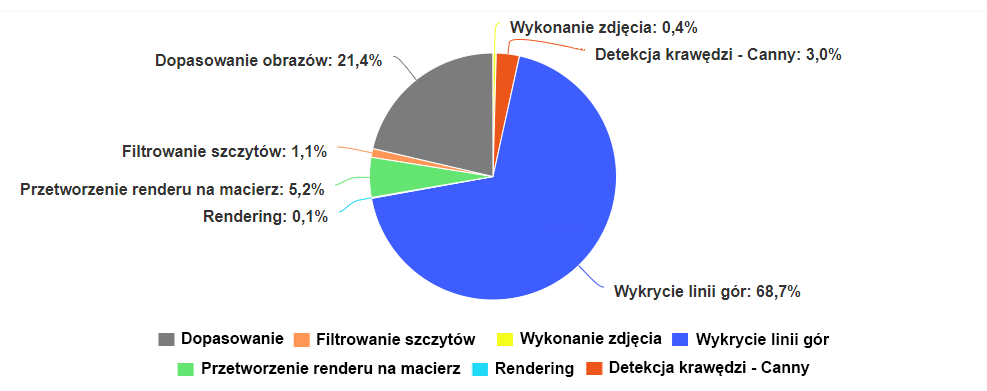
\includegraphics[width=0.9\linewidth]{img/pie_chart_profilowanie_przed_linii.png}
    \caption{Profilowanie procesu identyfikacji szczytów górskich przed optymalizacją wykrywania krawędzi najwyższych gór.}
    \label{fig:profilowanie_przed_linia}
\end{figure}


Z punktu widzenia człowieka oraz tego jak przetwarza on pewne dane, proces wybierania najwyższych krawędzi na danym obrazie binarnym powinien odbywać się kolumna po kolumnie, sprawdzając piksele od góry do dołu. W momencie natrafienia na biały punkt powinien on go wybrać i przejść do następnej kolumny. Takie podejście wydaje się logiczne z takiego punktu widzenia i w ten sposób najpierw został zaimplementowany ten etap. Jednak jest to sposób dobry tylko dla człowieka. 

Najczęstszą formą reprezentacji zdjęć w pamięci jest zapis rzędami. Oznacza to, że wartości pikseli w danym rzędzie są kolejnymi wpisami pamięci. Taki format występuje również w OpenCV \cite{opencv_mat}. W tym wypadku dla procesora lepszy jest dostęp do zdjęcia rzędami, ponieważ minimalizuje liczbę zapytań do pamięci i skoków między adresami odpowiednich komórek. Pozwala to również na wykorzystanie pamięci podręcznej CPU, ze względu na to, że może on pobrać i zapisać w niej pewną liczbę kolejnych pikseli. Nowoczesne procesory wyposażane są w tzw. prefetcher, który automatycznie wykrywa wzorce dostępu do pamięci i z wyprzedzeniem pobiera dane \cite{cache_memory}. Dzięki temu nie ma potrzeby ciągłego odpytywania pamięci RAM i przesyłania kolejnych informacji. Dodatkowo, dostęp do pamięci podręcznej w porównaniu do operacyjnej jest sporo szybszy \cite{memory_hierarchy}.

Takie rozważania teoretyczne potwierdza diagram \ref{fig:profilowanie_po_linia}. Po zmianie implementacji na analizę obrazu rzędami, wykrycie linii gór stanowi już jedynie $4\%$ czasu całego cyklu. Mimo, że w tym przypadku przetwarzane było całe zdjęcie, a nie tylko niektóre wartości w poszczególnych kolumnach. Możliwe jest dodatkowe zmniejszenie czasu przez zastosowanie flag logicznych celem opuszczenia pętli po znalezieniu wszystkich poszukiwanych pikseli. W przypadku pesymistycznym, gdy wszystkie potrzebne krawędzie będą znajdować się w~dolnej części zdjęcia, może pogorszyć to efektywność. Jednak możliwe jest założenie, że potencjalne oprogramowanie stworzone na podstawie opisywanego w niniejszej pracy dyplomowej procesu, będzie wykorzystywane w taki sposób, że krawędzie analizowanych gór będą znajdować się w środkowej części kadru. Dla tak umiejscowionych szczytów udział tego etapu w całym cyklu spada do $3\%$. 

\begin{figure}[!h]
    \centering 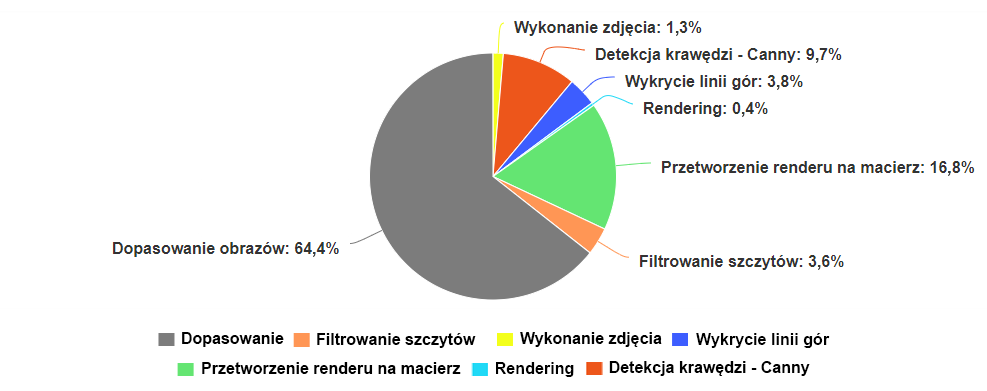
\includegraphics[width=0.9\linewidth]{img/pie_chart_profilowanie_po_linii.png}
    \caption{Profilowanie procesu identyfikacji szczytów górskich po optymalizacji wykrywania krawędzi najwyższych gór poprzez zmianę kolejności analizy pikseli i wykorzystaniem pamięci podręcznej.}
    \label{fig:profilowanie_po_linia}
\end{figure}

Po zmianie implementacji wykrywania linii gór, najwięcej czasu procesor poświęca na dopasowanie obrazów. Związane to jest z koniecznością wycinania obszaru dla każdego szczytu z obu obrazów binarnych, tworząc za każdym razem nowe macierze. Następnie przeprowadzana jest analiza dla każdego takiego fragmentu. Sumarycznie prowadzi to do dużej ilości obliczeń wykonywanych przez procesor. Z tego powodu prawdopodobnie poprawny jest tak duży procentowy udział tego etapu w cyklu detekcji szczytów. 

Analiza ta pokazuje, że odpowiednie przetwarzanie tablic wielowymiarowych oraz wykorzystanie pamięci podręcznej mogą być kluczowymi czynnikami wpływającymi na złożoność czasową danego zagadnienia. Można też wyciągnąć z tego wnioski, że reprezentacja w pamięci danych dwu i więcej wymiarowych w sposób ciągły pozwala zoptymalizować do nich dostęp i zmniejszyć liczbę potrzebnych zapytań. Zasadne wydaje się w takich przypadkach pisanie kodu w sposób zorientowany na optymalizację nawet kosztem czytelności i refaktoringu czy nawet logiczności i zgodności z ludzką intuicją.